\documentclass[aspectratio=169,xcolor=dvipsnames, t]{beamer}

\usepackage{cp24}
\usepackage[square,numbers]{natbib}

\bibliographystyle{ACM-Reference-Format}

%*************************************************************************************************************
\title[Customizable Roundtrips with Tour4Me]{Customizable Roundtrips with Tour4Me}
\subtitle{Meta-heuristic Approaches for Personalized Running and Cycling Routes}
\author[Lisa Salewsky]{
	Lisa Salewsky
}


\institute[TU Dortmund]{
	\begin{minipage}[t][2.3cm][b]{0.7\textwidth}
		\centering
		\begin{tikzpicture}[remember picture,overlay]
			\node[inner sep=0] at (2.5,-0.8) {\includegraphics[scale=0.1]{logo.png}};
		\end{tikzpicture}
		TU Dortmund, Fakultät für Informatik\\
		\vspace{1.5cm}
		Reviewer:\\
		Prof. Dr. Kevin Buchin\\
		Mart Hagedoorn, M. Sc.
	\end{minipage}
	
}
\date[\today]{\today}
\beamertemplatenavigationsymbolsempty %Navigantionszeite unten aus
%*************************************************************************************************************
%\usetheme{Malmoe} 
%\usetheme{Madrid}
%\usecolortheme{rose} %schwache farben
% Themes:
%AnnArbor | Antibes | Bergen |Berkeley | Berlin | Boadilla |boxes | CambridgeUS | Copenhagen |Darmstadt | default | Dresden |
%Frankfurt | Goettingen |Hannover | Ilmenau | JuanLesPins | Luebeck | Madrid | Malmoe | Marburg |
%Montpellier | PaloAlto | Pittsburgh |Rochester | Singapore | Szeged |Warsaw
\useinnertheme{rounded}
%\useoutertheme{shadow} %schattierung in den Rechtecken der Blocken -- nix
%*************************************************************************************************************


% Customize the table of contents
\setbeamertemplate{section in toc}[square]
\setbeamertemplate{subsection in toc}[square]
\setbeamertemplate{section/subsection in toc}[square]
\setbeamercolor{section number projected}{bg=tu_green_full,fg=white}
\setbeamercolor{subsection number projected}{bg=tu_green_full,fg=white}

% Customize all the bulletpoints
\setbeamertemplate{items}[square]

% Customize the link colors
\hypersetup{
	colorlinks=true,
	linkcolor=tu_green_full2,
	urlcolor=tu_green_full2,
	citecolor=tu_green_full2
}

\setbeamercolor{block title}{bg=tu_light_green_full2, fg=black}
\setbeamercolor{block body}{bg=tu_light_green_full3, fg=black}


\begin{document}
	%*************************************************************
	\begin{frame}
		\thispagestyle{empty}
		\titlepage
	\end{frame}
	%*************************************************************
%	
%	\begin{frame}{Agenda}
%		\centering	
%		\tableofcontents
%	\end{frame}
	
	\section{Einleitung}
	
	\begin{frame}{Einleitung}
		\vspace{0.25cm}
		Warum eine App zum Erstellen von Rundrips?
		\only<2>{	
			\begin{figure}
				\includegraphics[height=0.6\textheight]{images/IMG-20231124-WA0010-cropped.jpg}
			\end{figure}}
		\only<3>{	
			\begin{figure}
				\includegraphics[height=0.6\textheight]{images/IMG-20231124-WA0039-cropped.jpg}
			\end{figure}}
		\only<4>{	
			\begin{figure}
				\includegraphics[height=0.6\textheight]{images/WhatsApp Bild 2023-11-24 um 14.35.53_5752c78a.jpg}
			\end{figure}}
	\end{frame}
	\begin{frame}{Einleitung}
		\vspace{0.25cm}
		Warum eine App zum Erstellen von Rundrips?
		\begin{columns}
			\begin{column}{0.48\textwidth}
				\includegraphics[height=0.3\textheight]{images/IMG-20231124-WA0010-cropped.jpg}
			\vspace{-1.5cm}
				\begin{flushright}
					\includegraphics[height=0.3\textheight]{images/IMG-20231124-WA0039-cropped.jpg}
				\end{flushright}
			\vspace{-1cm}
				\begin{flushleft}
					\includegraphics[height=0.3\textheight]{images/WhatsApp Bild 2023-11-24 um 14.35.53_5752c78a.jpg}
				\end{flushleft}
		\end{column}
		\pause
		\begin{column}{0.48\textwidth}
			\vspace{-2cm}
			\begin{block}{Gemeinsamkeiten}
				\begin{itemize}[<+->]
					\item Kann von A nach B gehen
					\item In der Freizeit aber oft Rundtrips
					\item Möglichst "hübsche" Routen mit zusätzlichen individuellen Wünschen gewünscht
				\end{itemize}
			\end{block}
		\end{column}
		\end{columns} ~\\
		
	\end{frame}
	
	\begin{frame}{Einleitung}
	\vspace{0.25cm}
	Warum eine App zum Erstellen von Rundrips?
	\pause
	\begin{itemize}[<+->]	
		\item viele Lösungen für kürzeste Wege von A nach B
		\item Optimieren alltägliche Routen
		\item Joggen und Radfahren in der Freizeit:
		\item weitere Bedingungen für attraktive Strecken nötig
		\item aber kaum Ansätze für Rundtrips mit Präferenzen
	\end{itemize}
	\end{frame}

	\begin{frame}{Einleitung}
		\vspace{0.25cm}
		Was macht eine Strecke attraktiv?\\
		\pause
		\vspace{-0.2cm}
		\begin{minipage}[t]{0.48\textwidth}
			\begin{itemize}[<+->]
				\item abhängig von individuellen Bedürfnissen und vom Level der Person
				\item viele verschiedene Faktoren
				\begin{itemize}[<+->]
					\item Wegtyp (Straße, Waldpfad, Radweg etc.)
					\item Untergrund (Teer, Kies, Sand, Erde, etc.)
					\item Steigung
					\item Umgebung (Wald, Park, Wohngegend, etc.)
					\item Form (Rund, gerade mit U-Turn, viele Abzweigungen, etc.)
				\end{itemize}
				\item Einfluss dieser auf Strecke individuell auswählen 
		\end{itemize}
		\end{minipage}
		\begin{minipage}[t][0.7\textheight][b]{0.48\textwidth}
			\only<4>{
				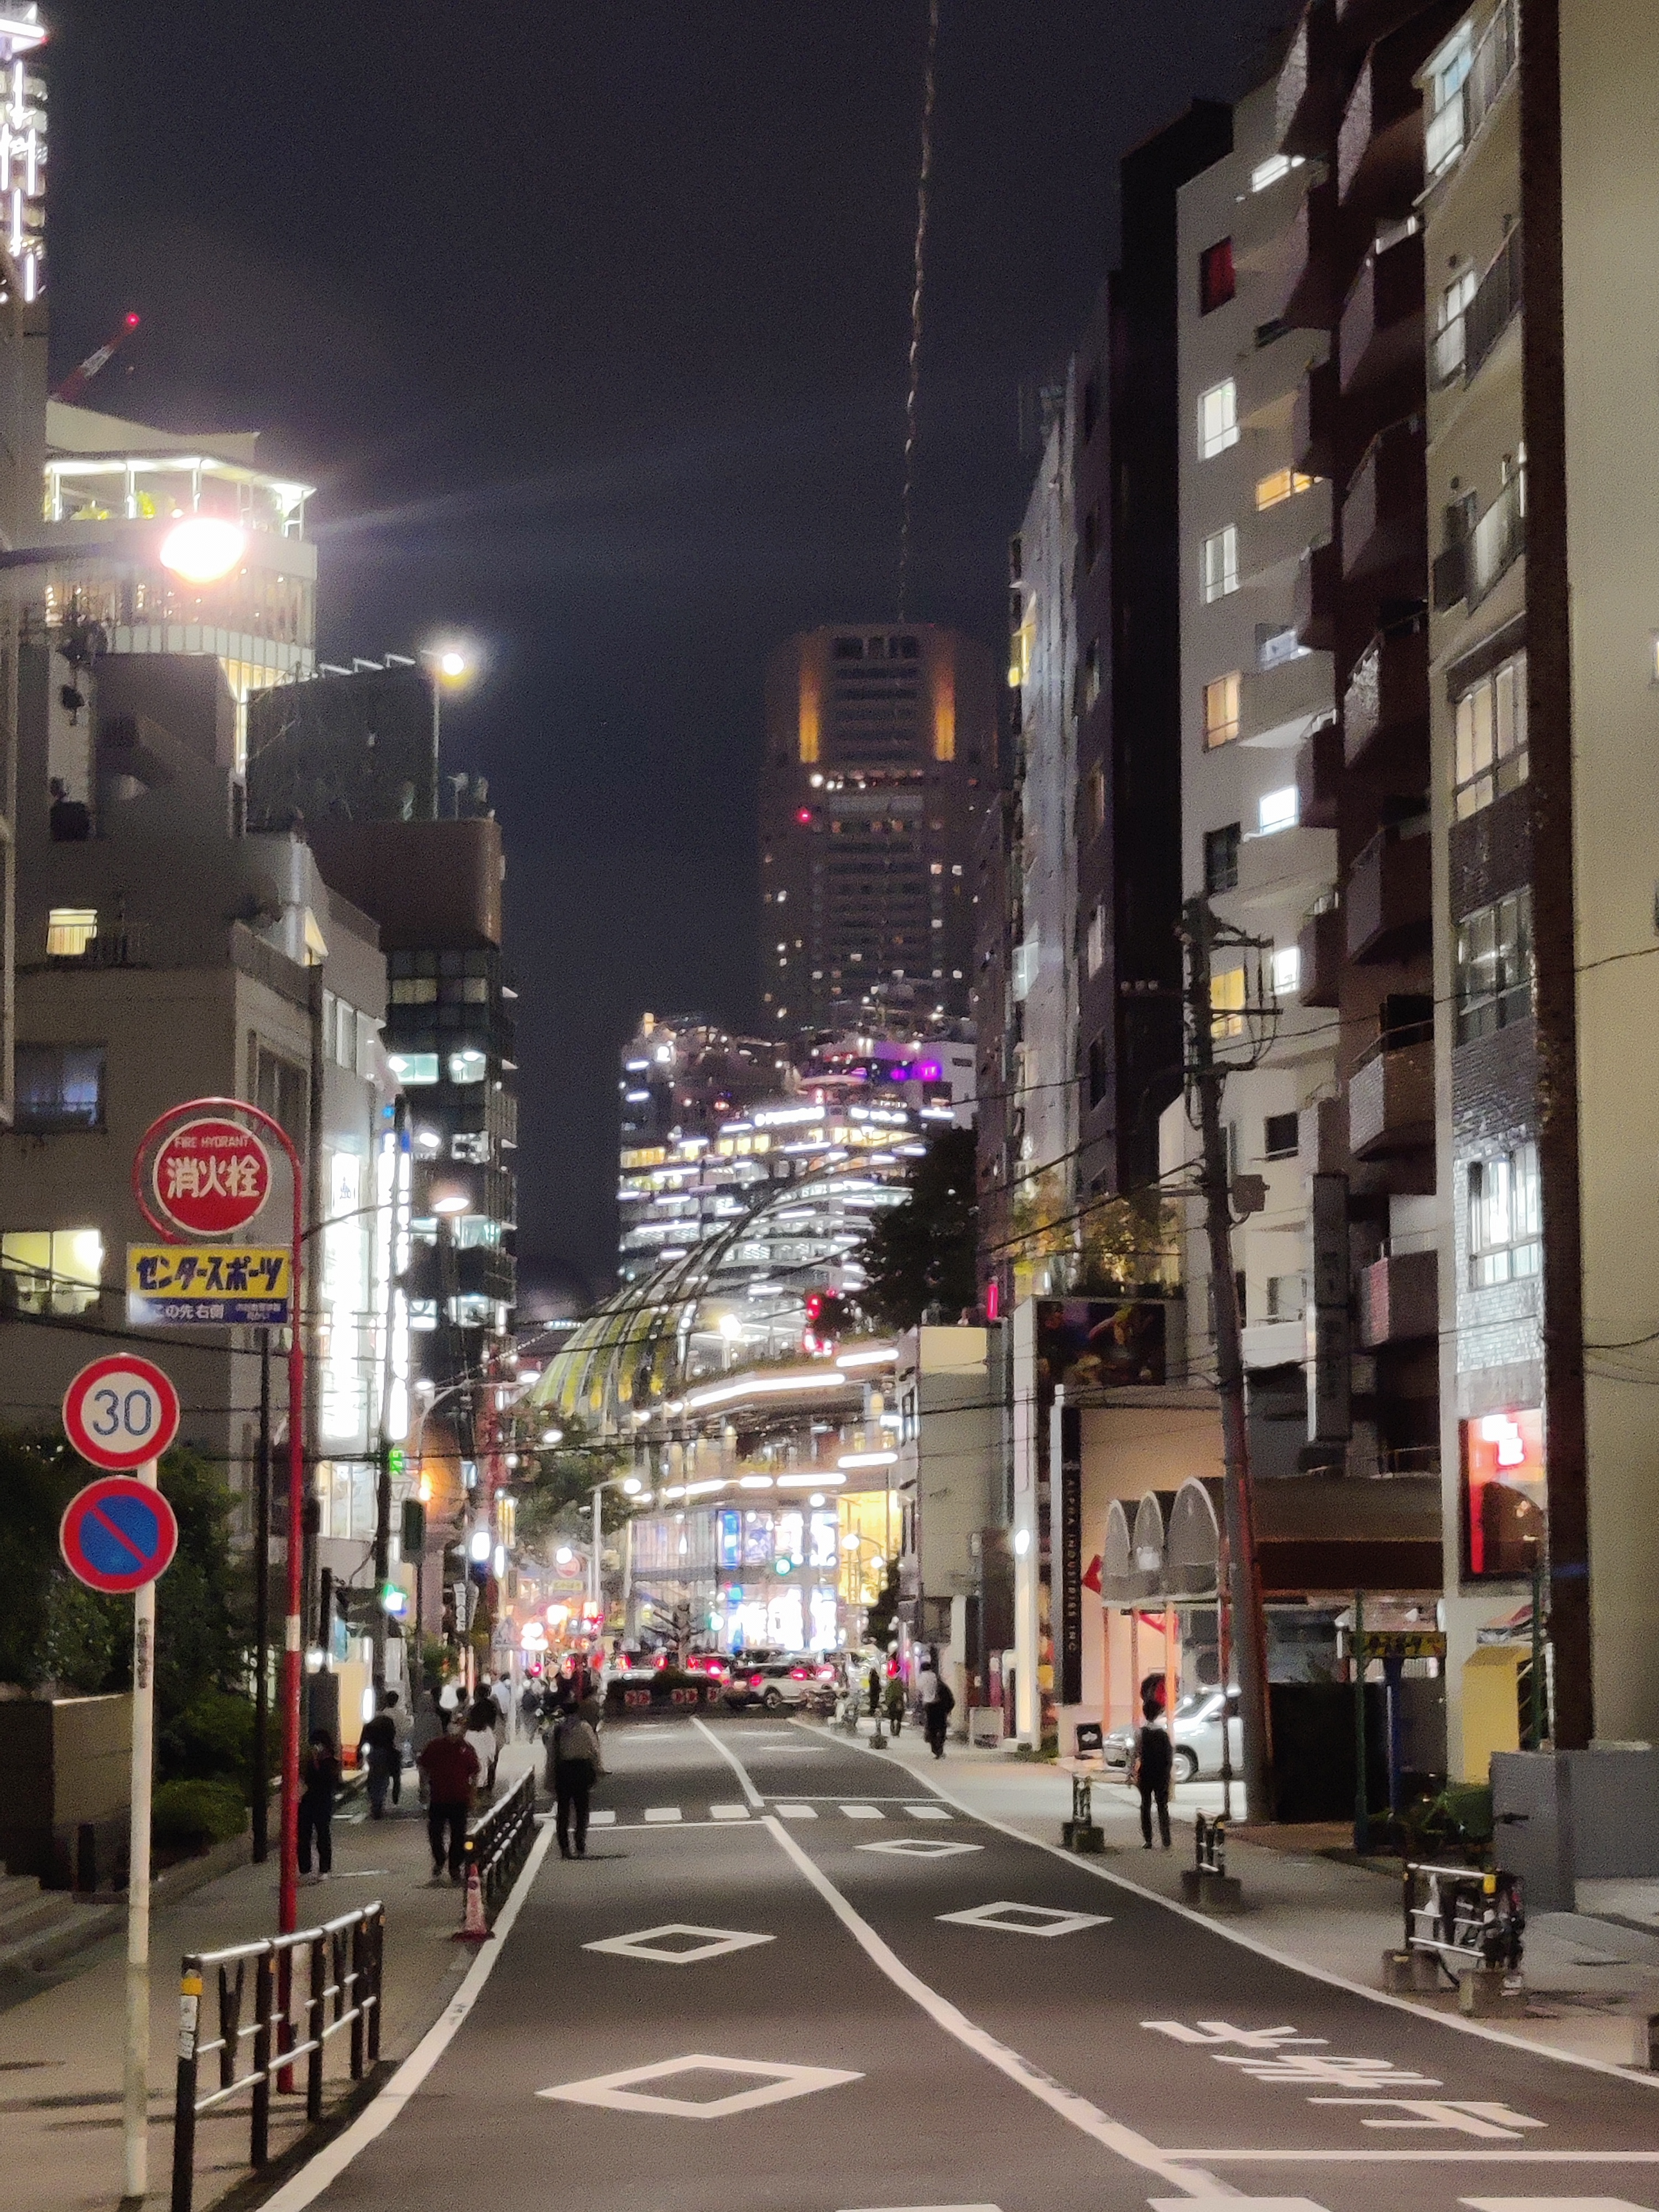
\includegraphics[height=0.5\textheight]{images/IMG_20220921_181918.jpg}
				\vspace{-3.5cm}
				\begin{flushright}
					\includegraphics[height=0.5\textheight]{images/IMG-20231124-WA0038.jpg}
				\end{flushright}
				\vspace{-1cm}
				\begin{flushleft}
					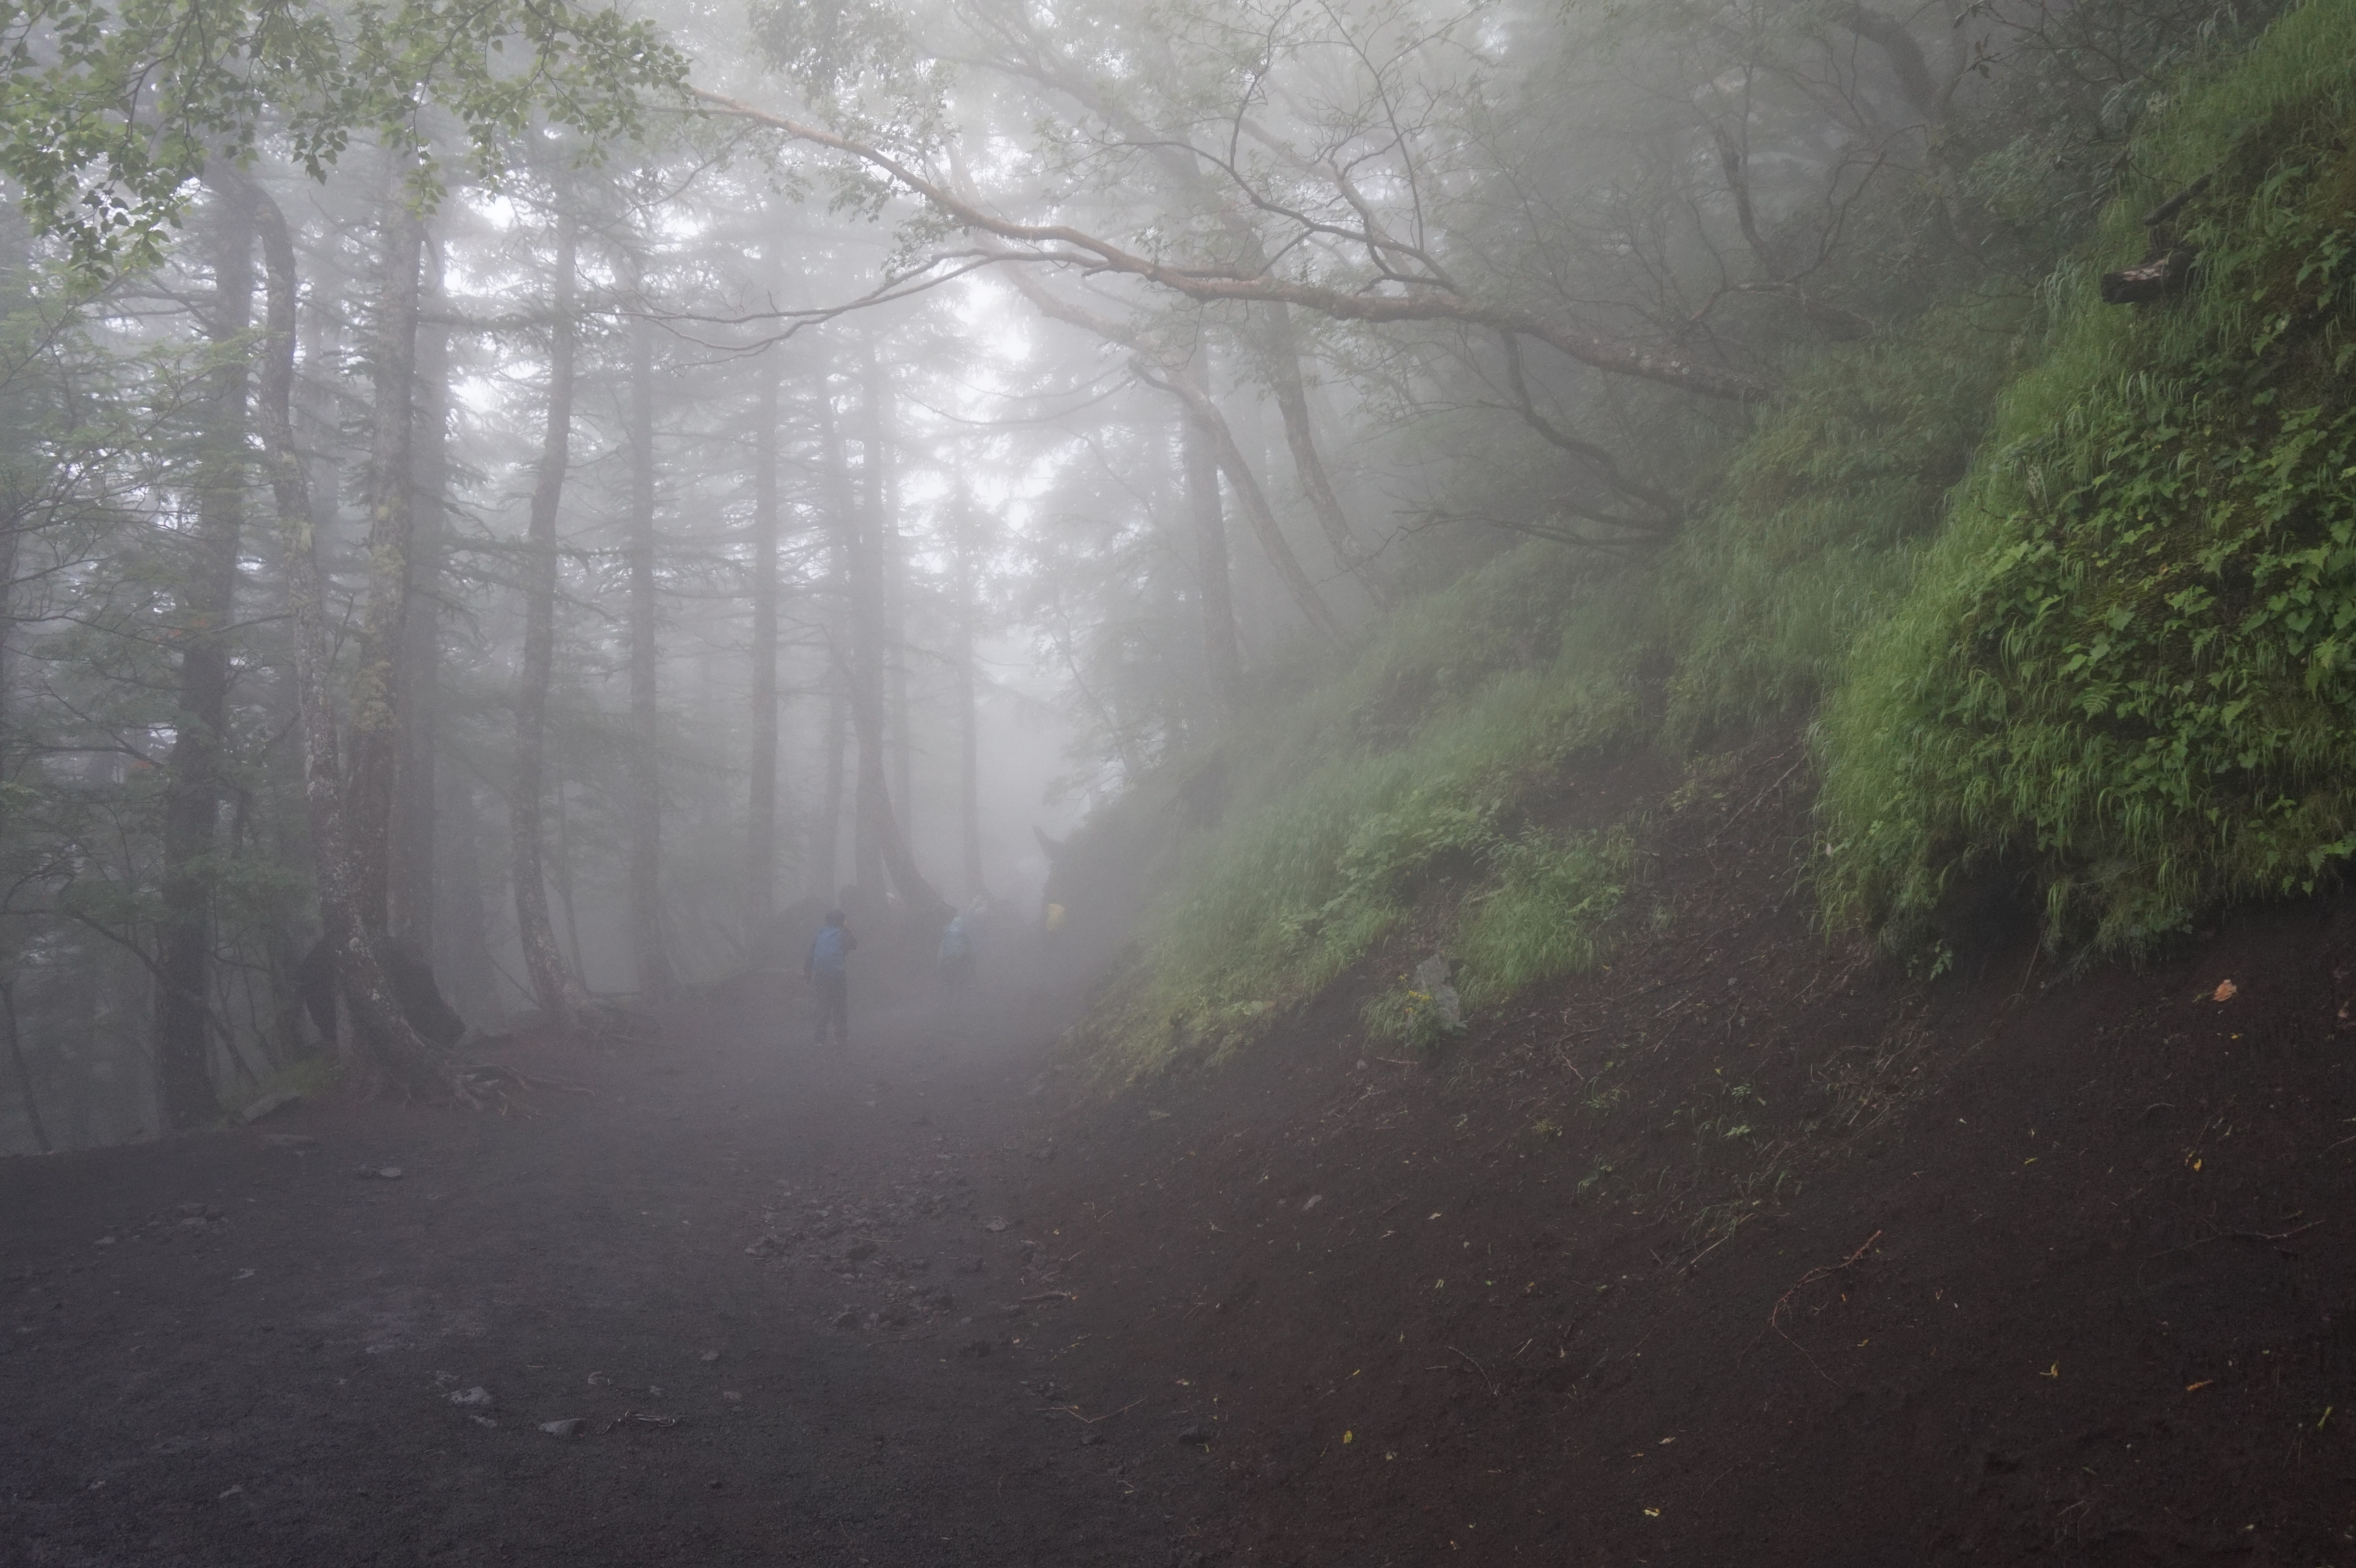
\includegraphics[height=0.3\textheight]{images/DSC00708.JPG}
				\end{flushleft}}
			\only<5>{
				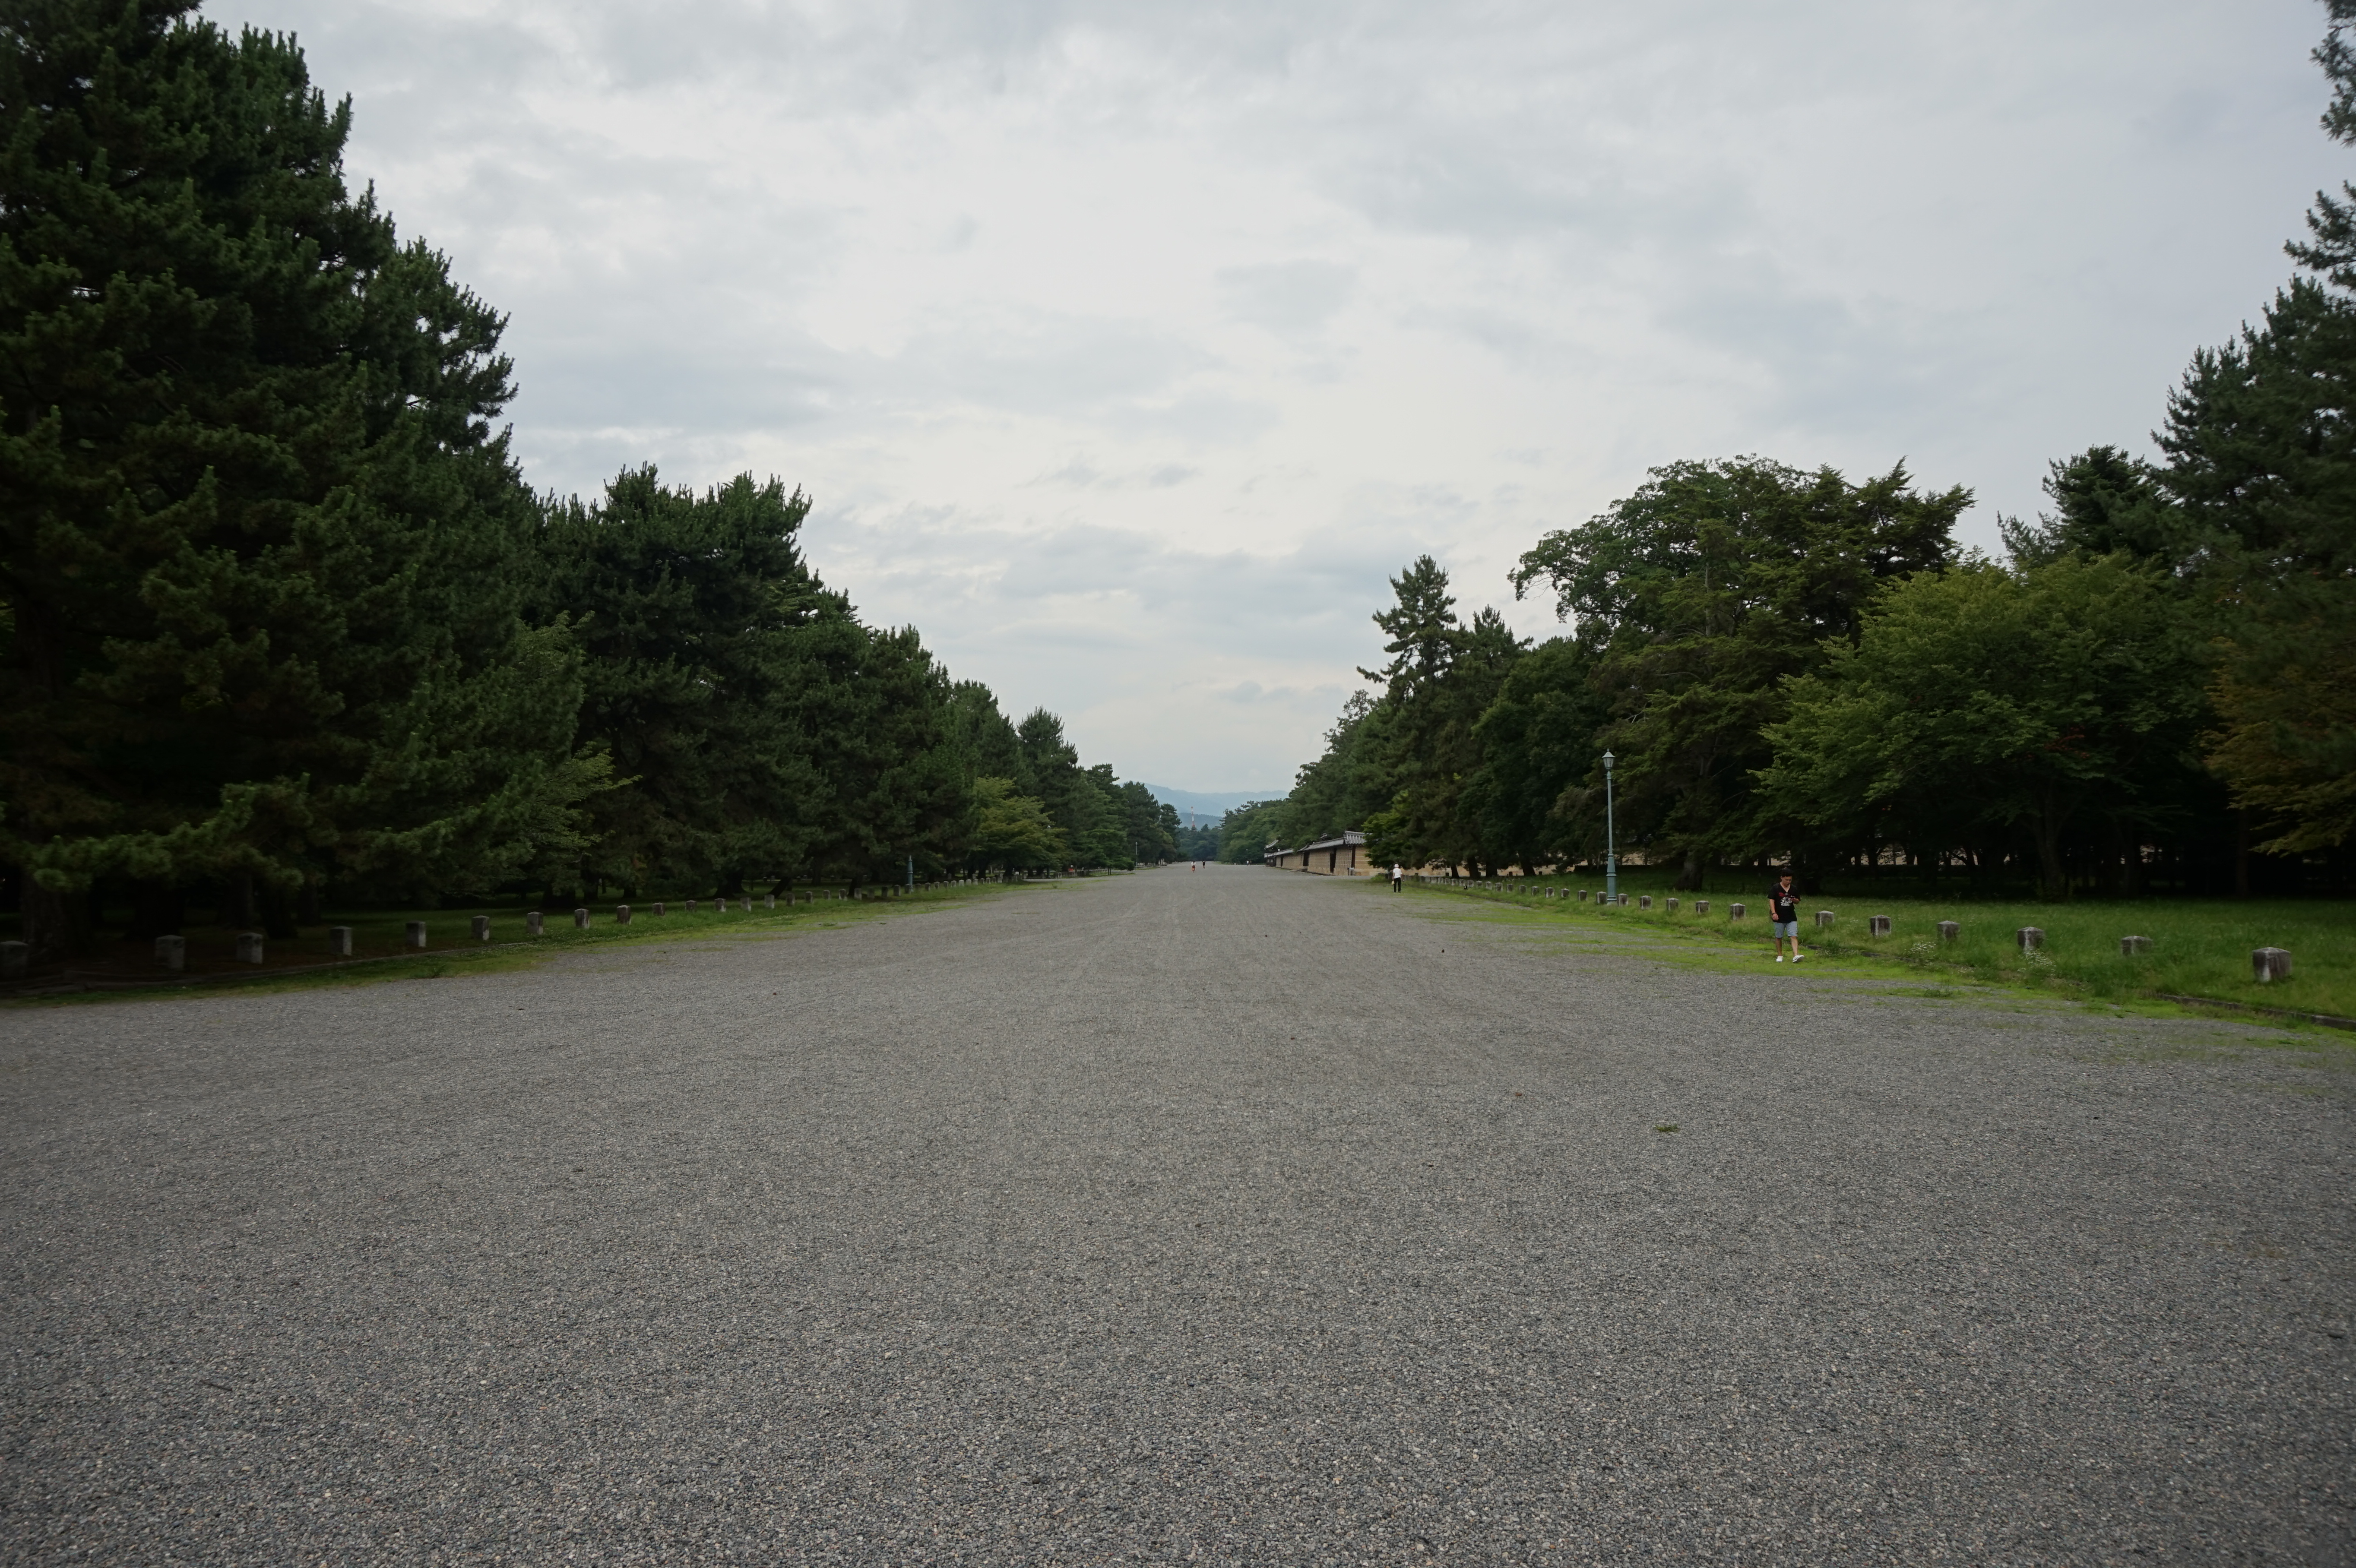
\includegraphics[height=0.3\textheight]{images/DSC08658.JPG}
				\vspace{-2cm}
				\begin{flushright}
					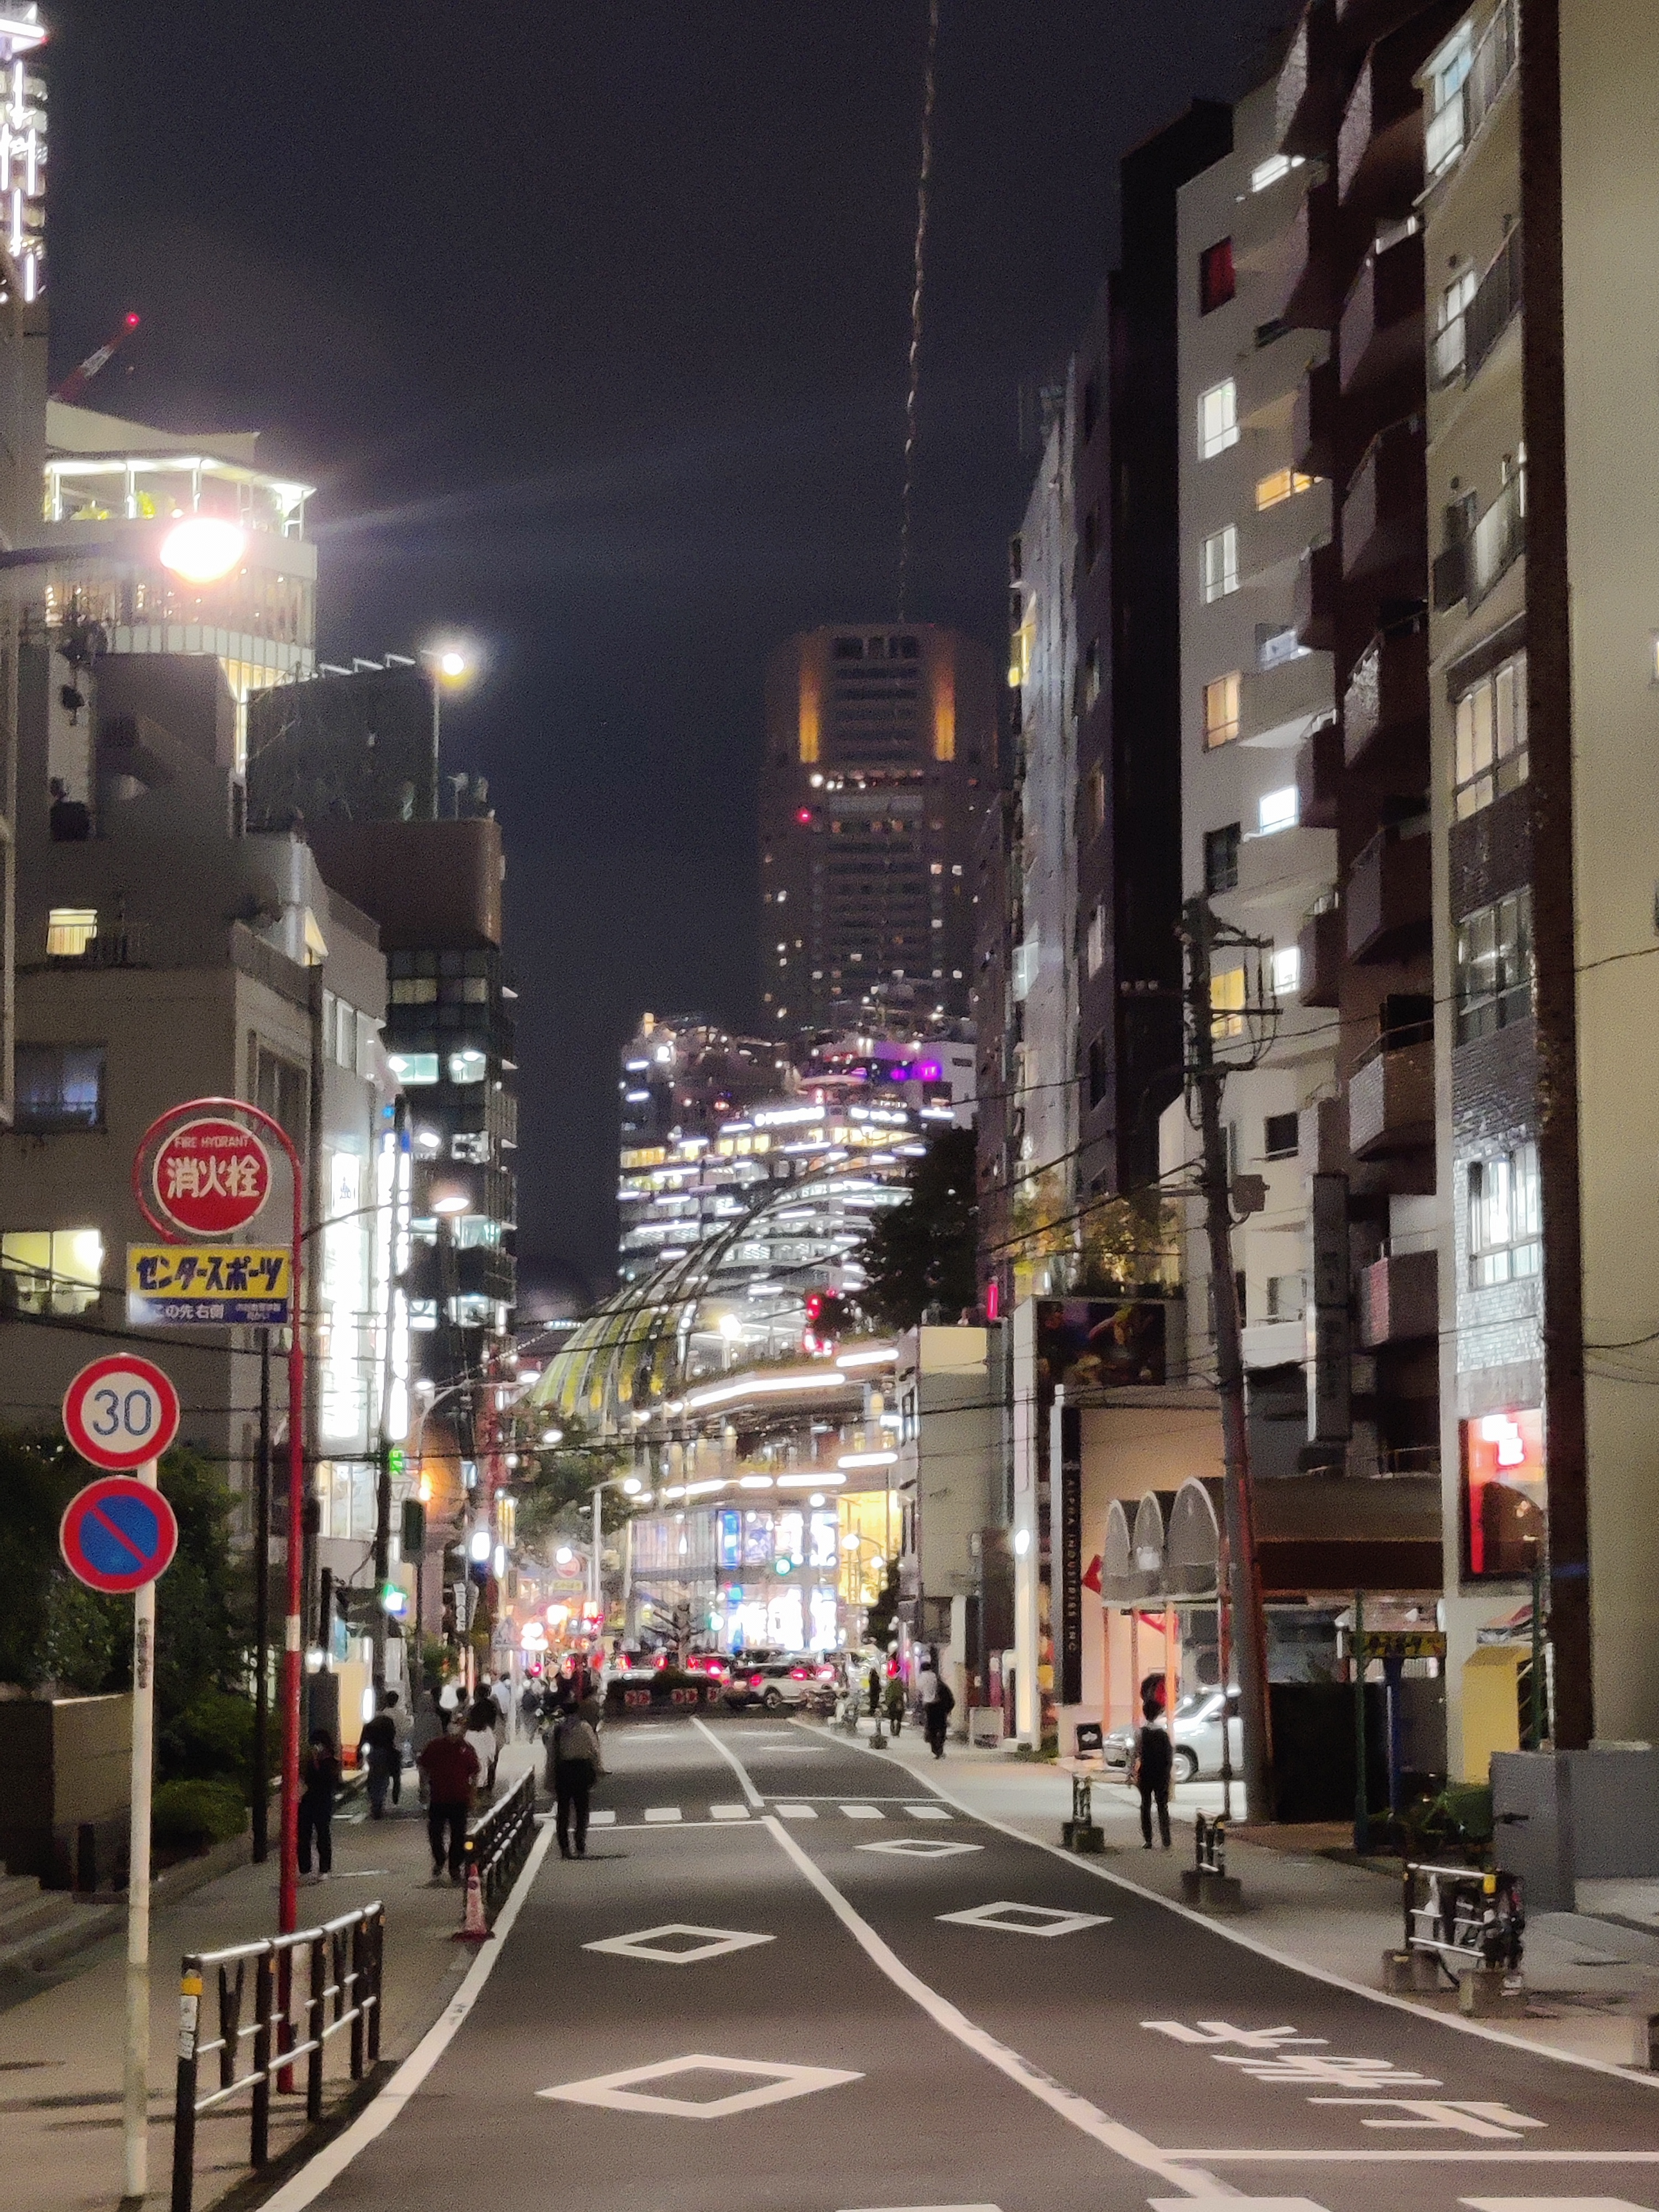
\includegraphics[height=0.5\textheight]{images/IMG_20220921_181918.jpg}
				\end{flushright}
				\vspace{-2cm}
				\begin{flushleft}
					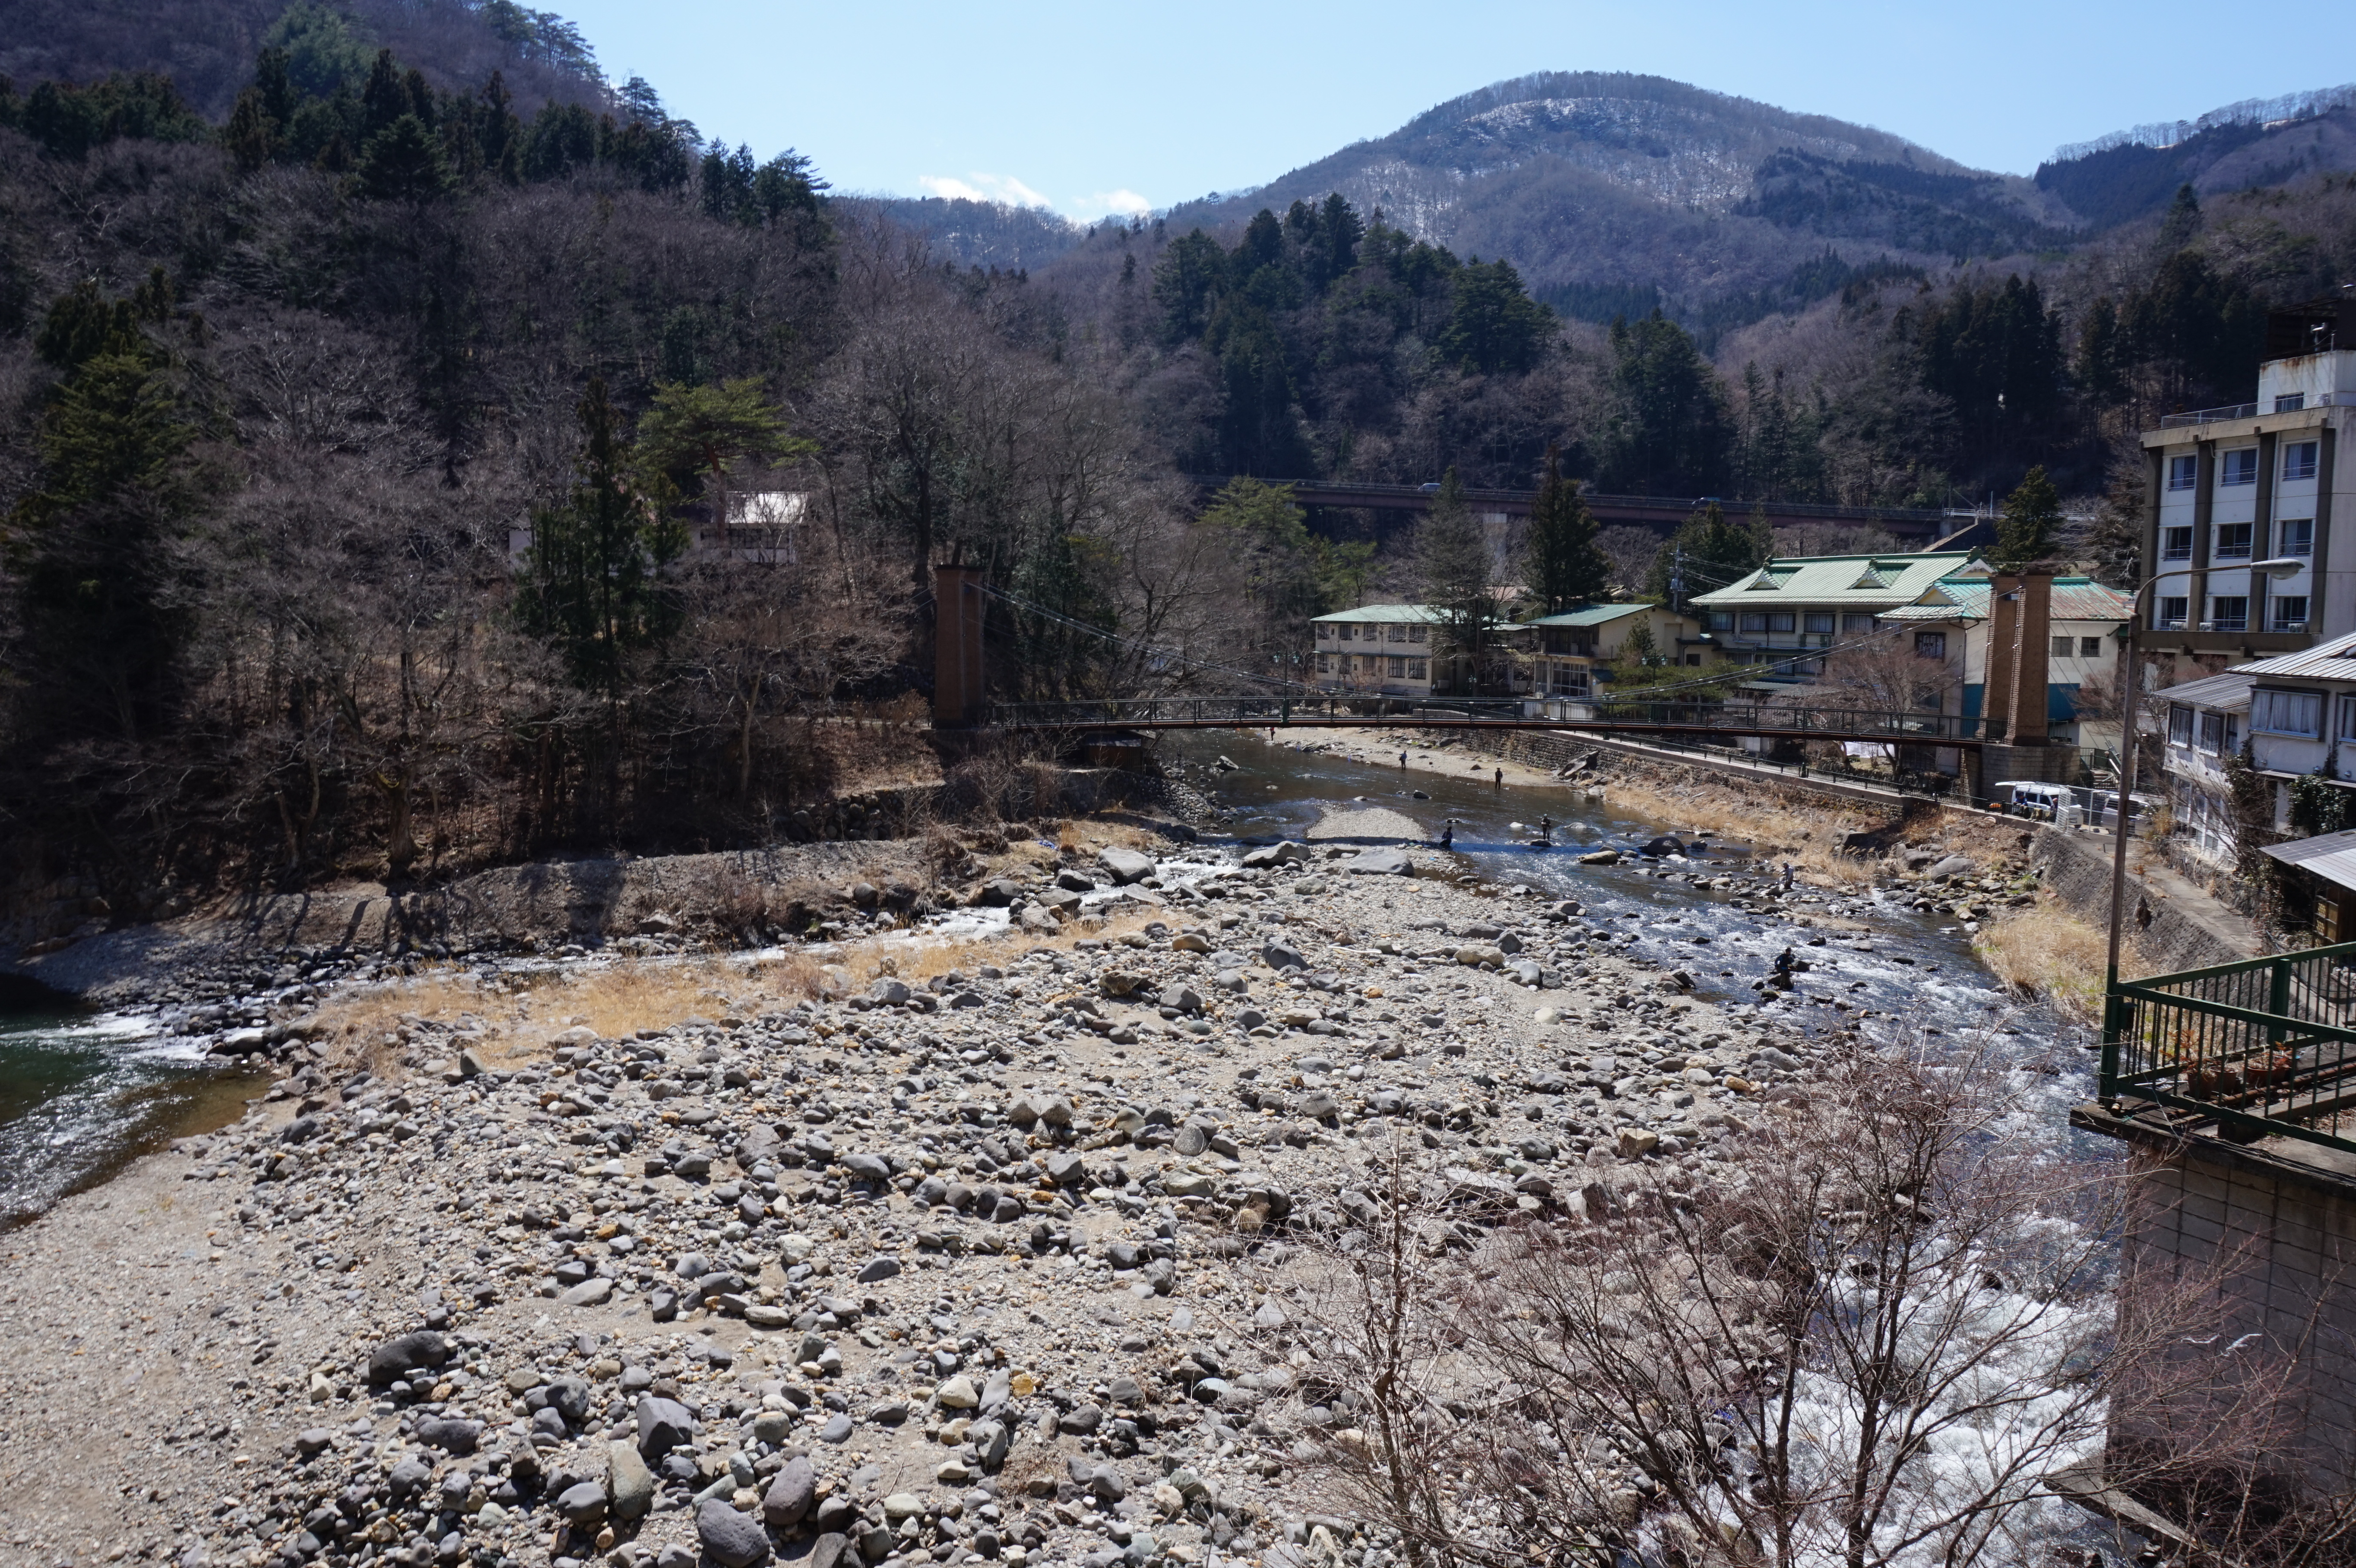
\includegraphics[height=0.3\textheight]{images/DSC03182.JPG}
				\end{flushleft}}
			\only<6>{
				\includegraphics[height=0.3\textheight, angle=90]{images/DSC00758.JPG}
				\vspace{-3cm}
				\begin{flushright}
					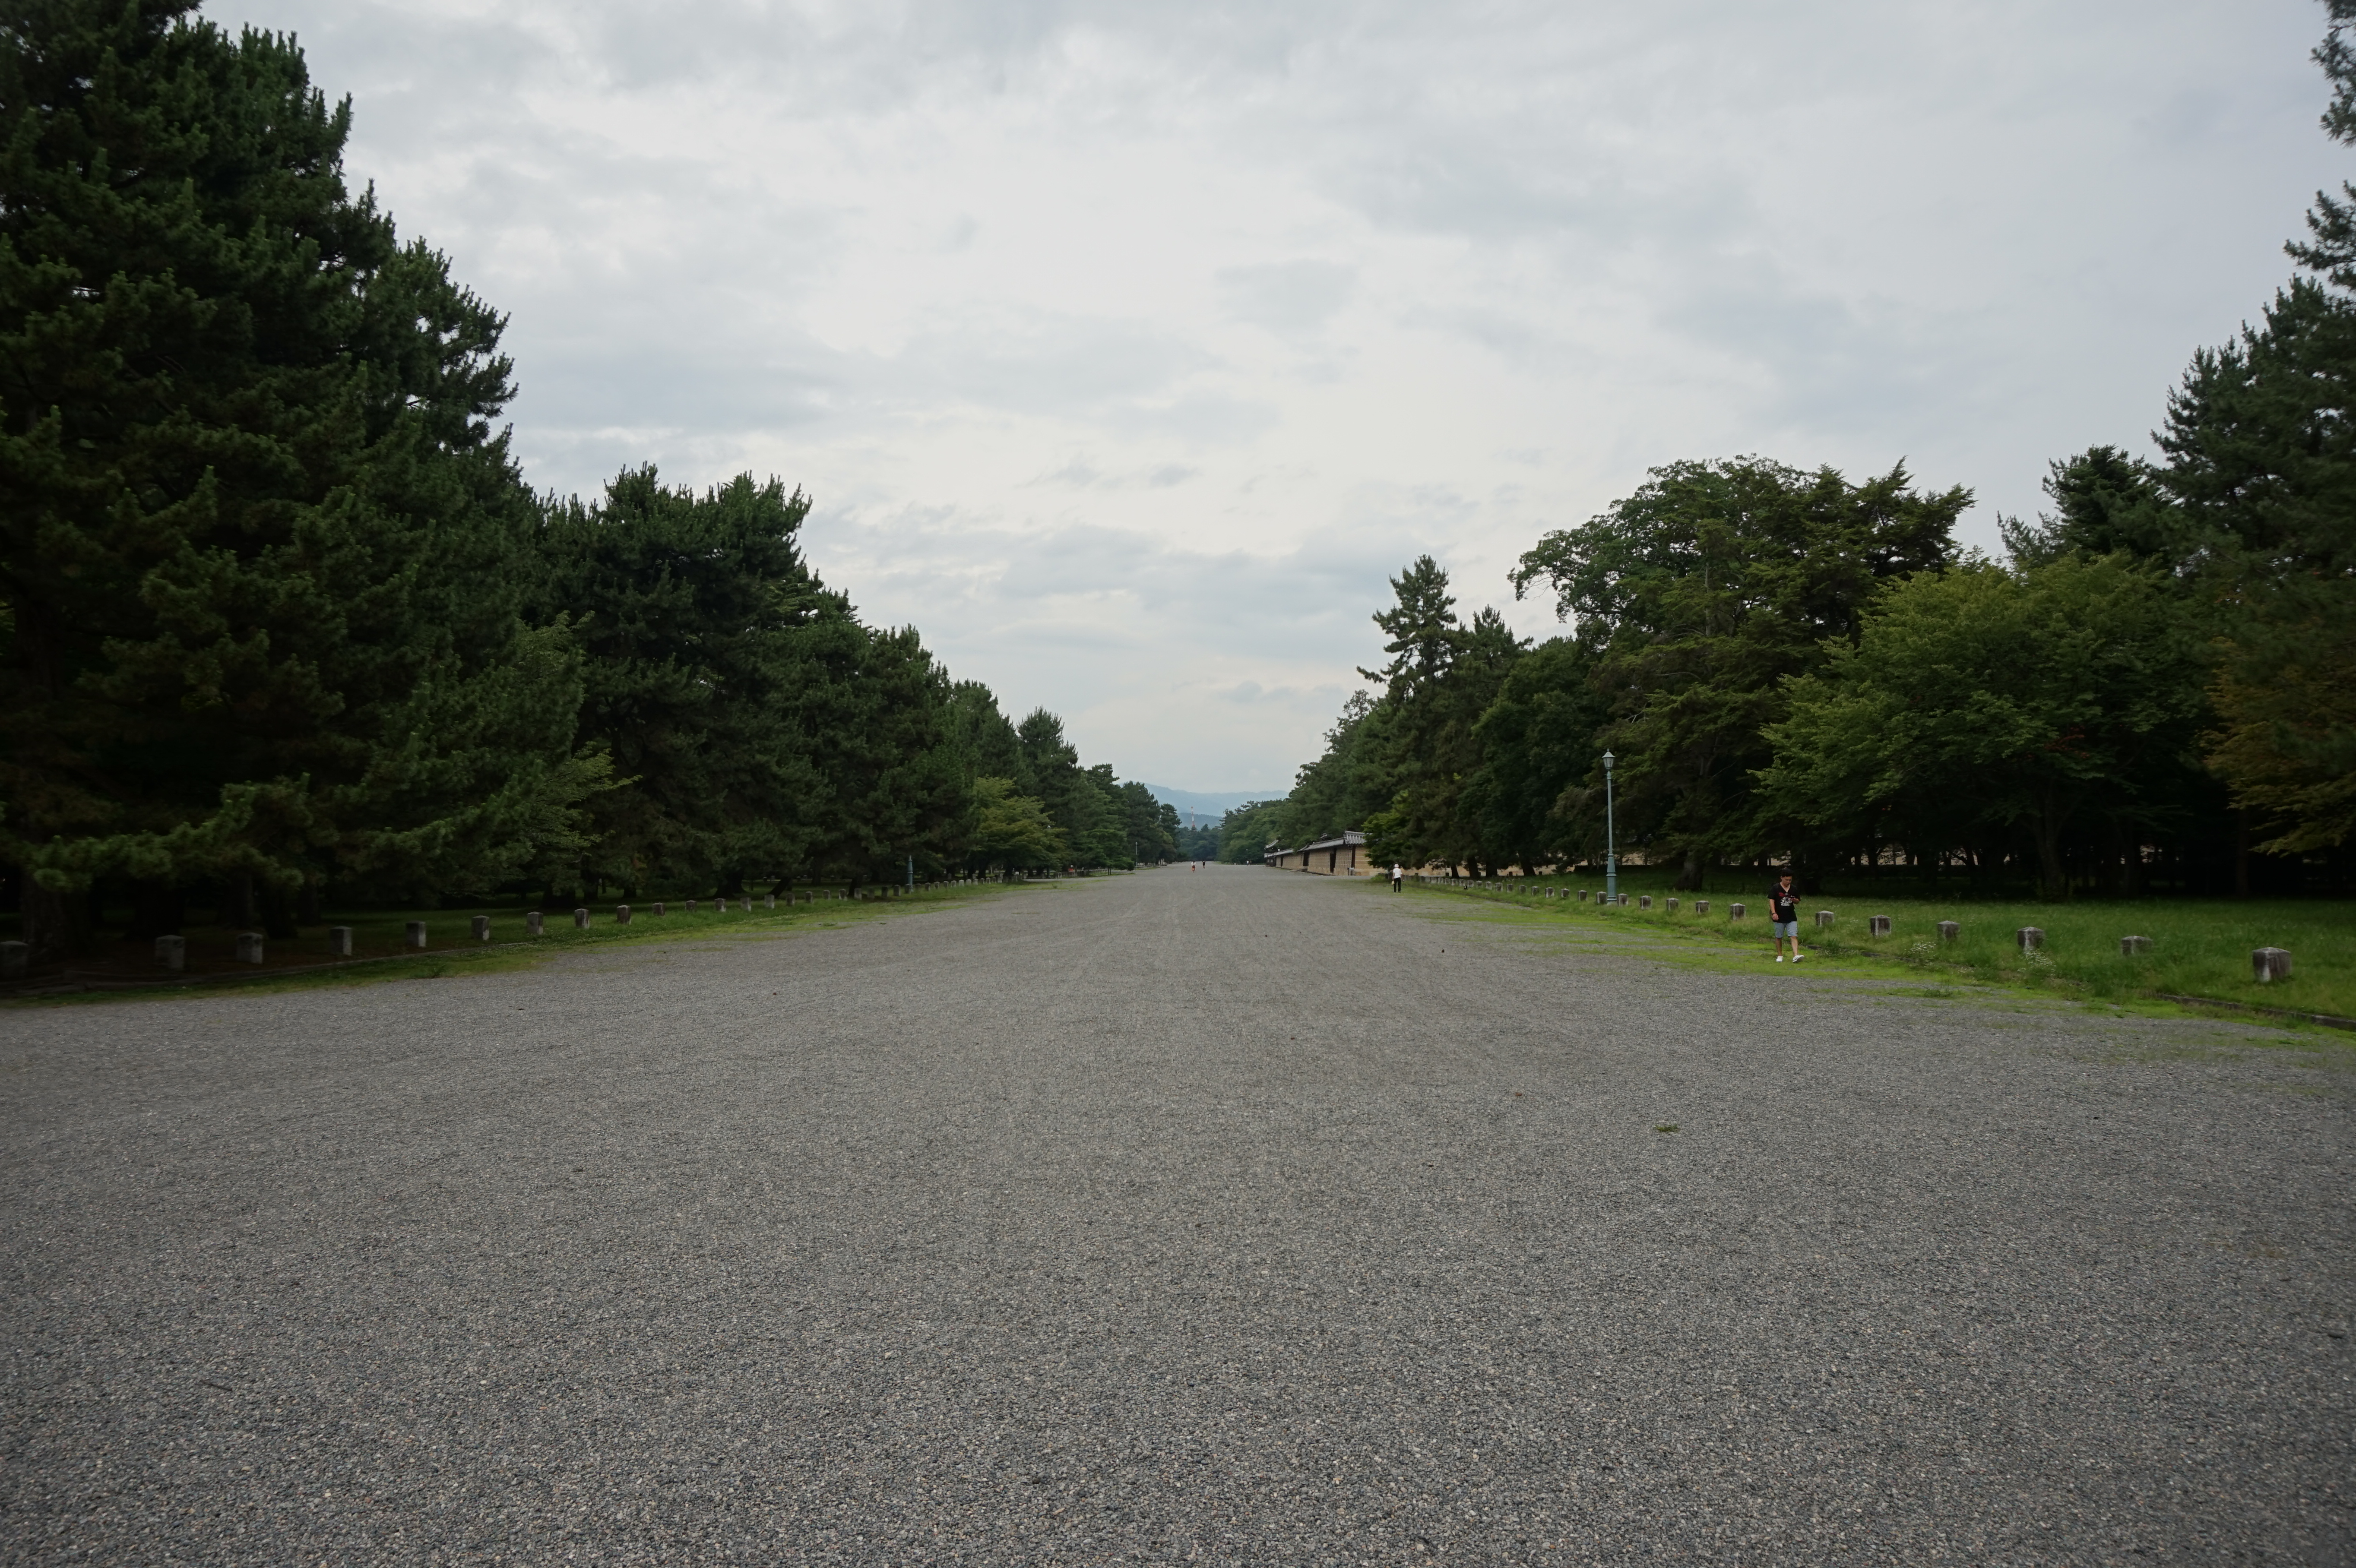
\includegraphics[height=0.3\textheight]{images/DSC08658.JPG}
				\end{flushright}
%				\vspace{0.5cm}
				\begin{flushleft}
					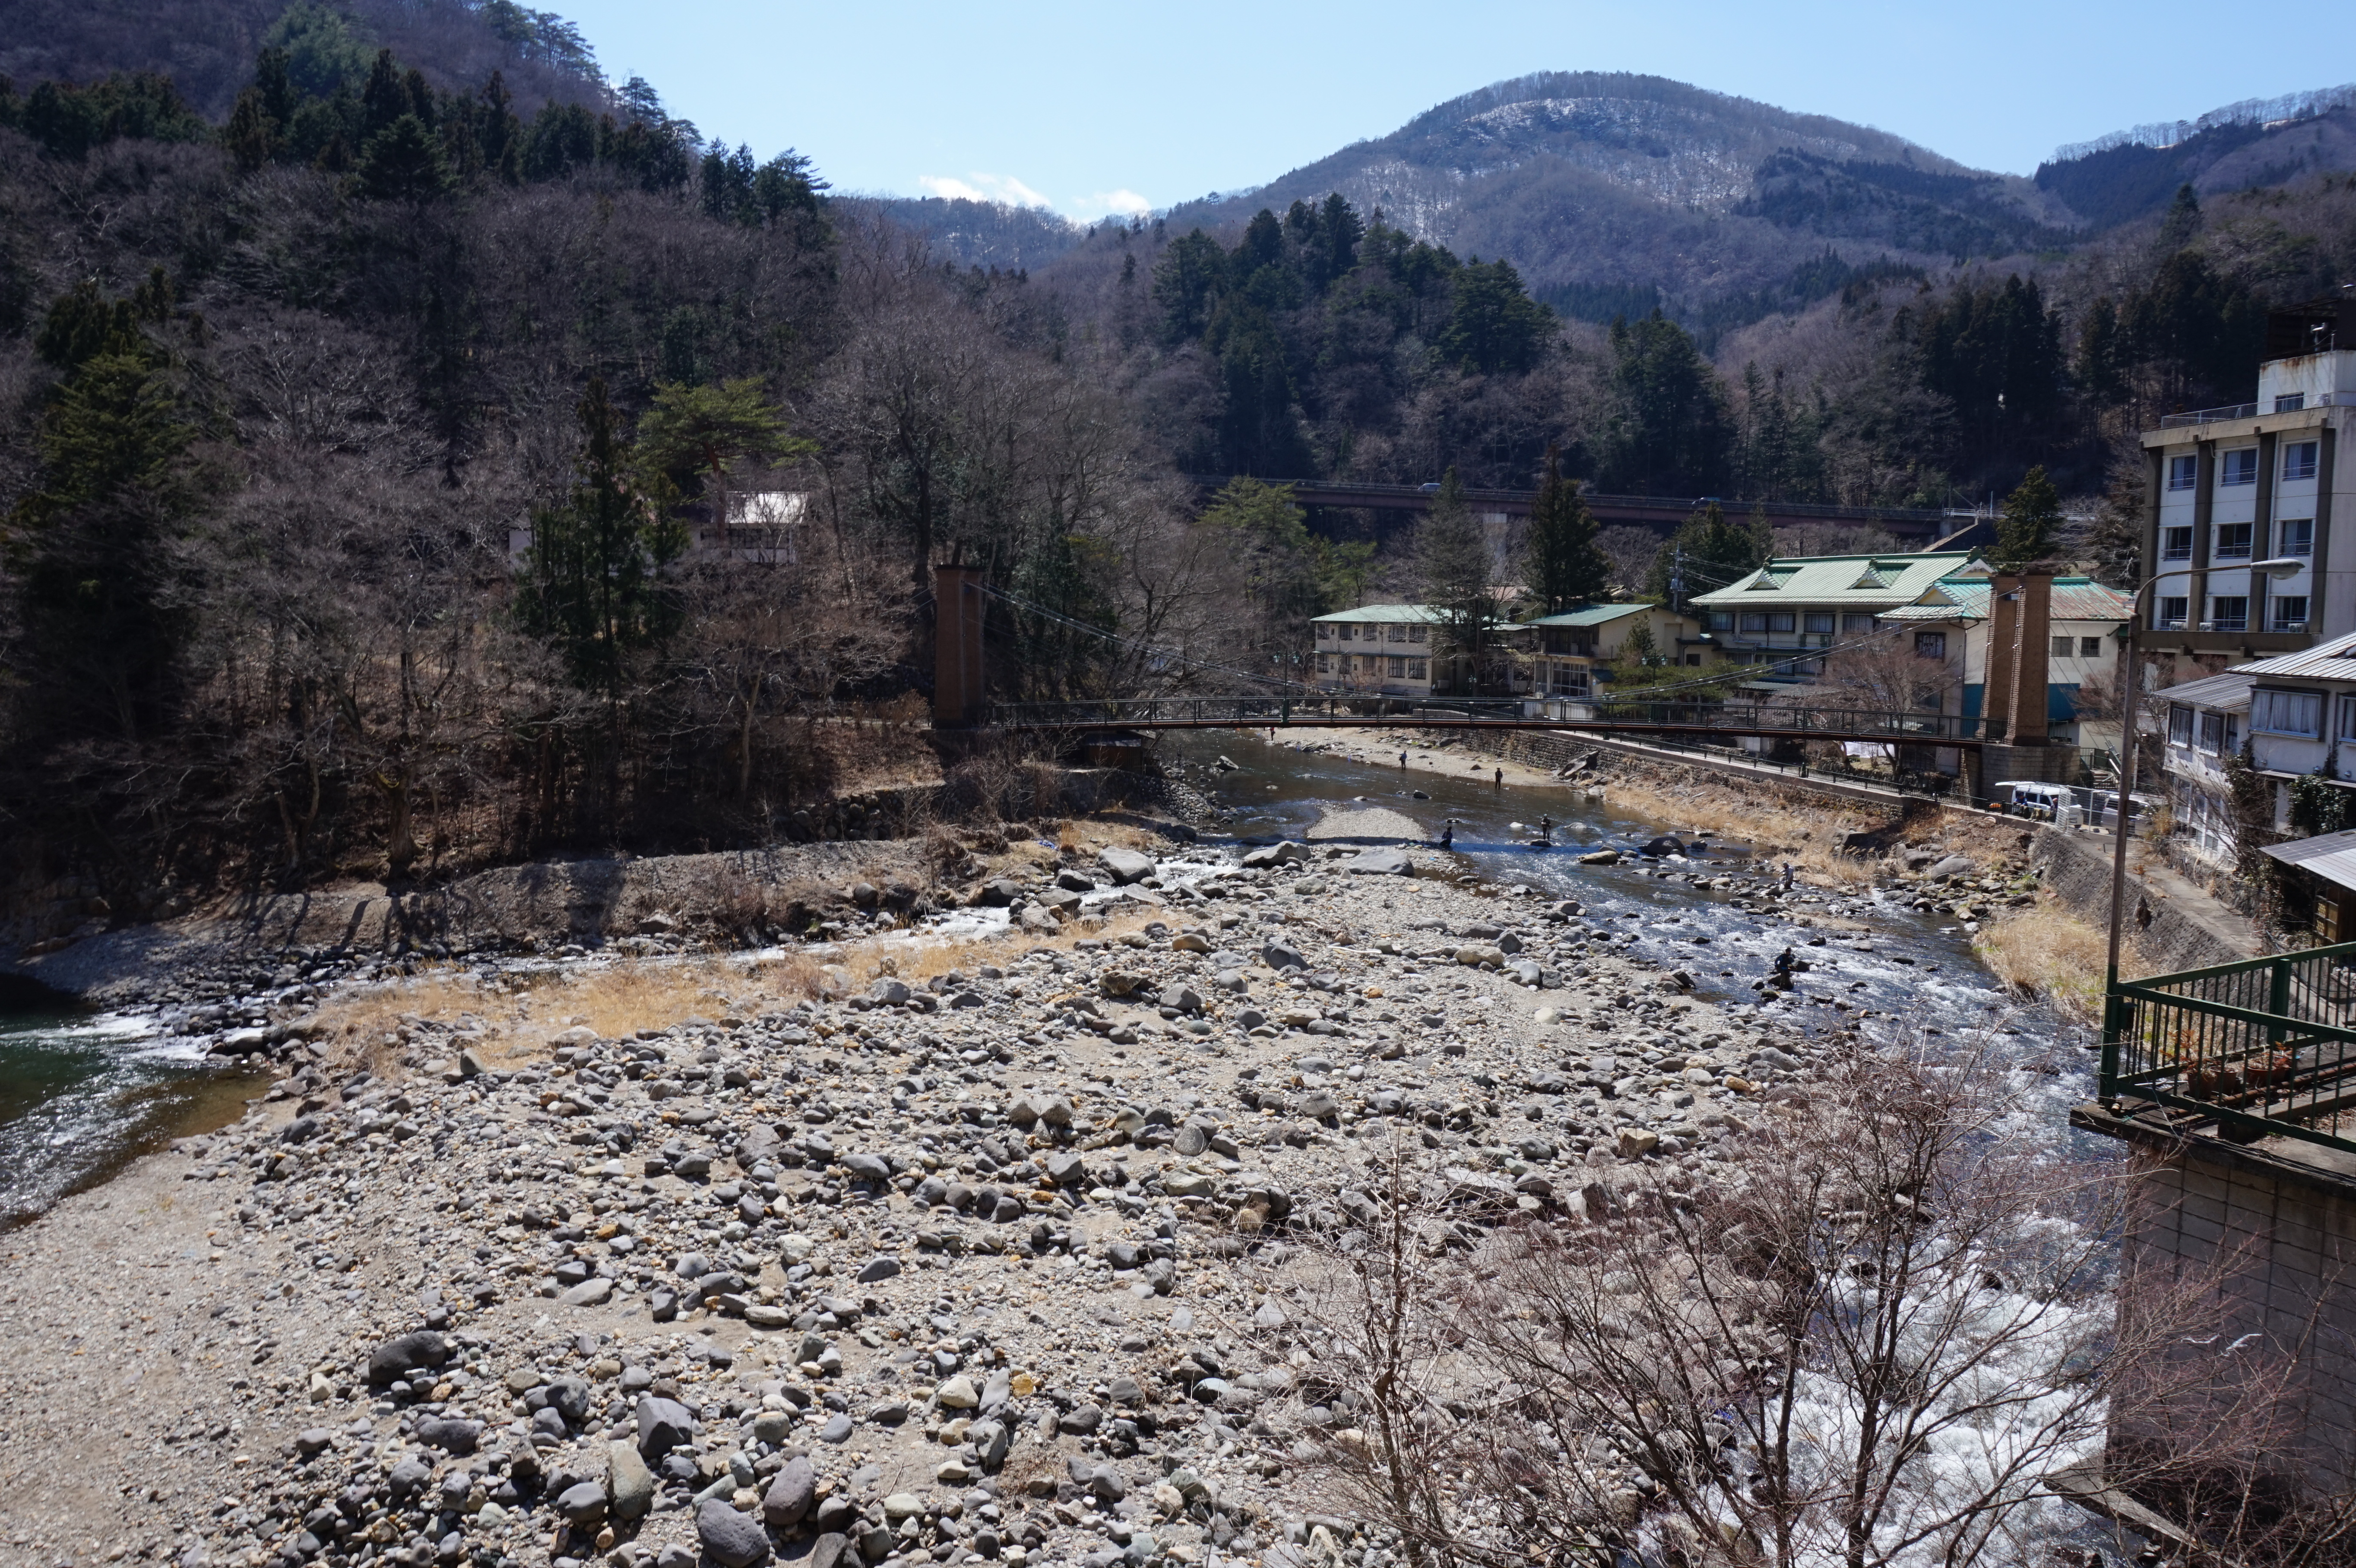
\includegraphics[height=0.3\textheight]{images/DSC03182.JPG}
				\end{flushleft}}
			\only<7>{
				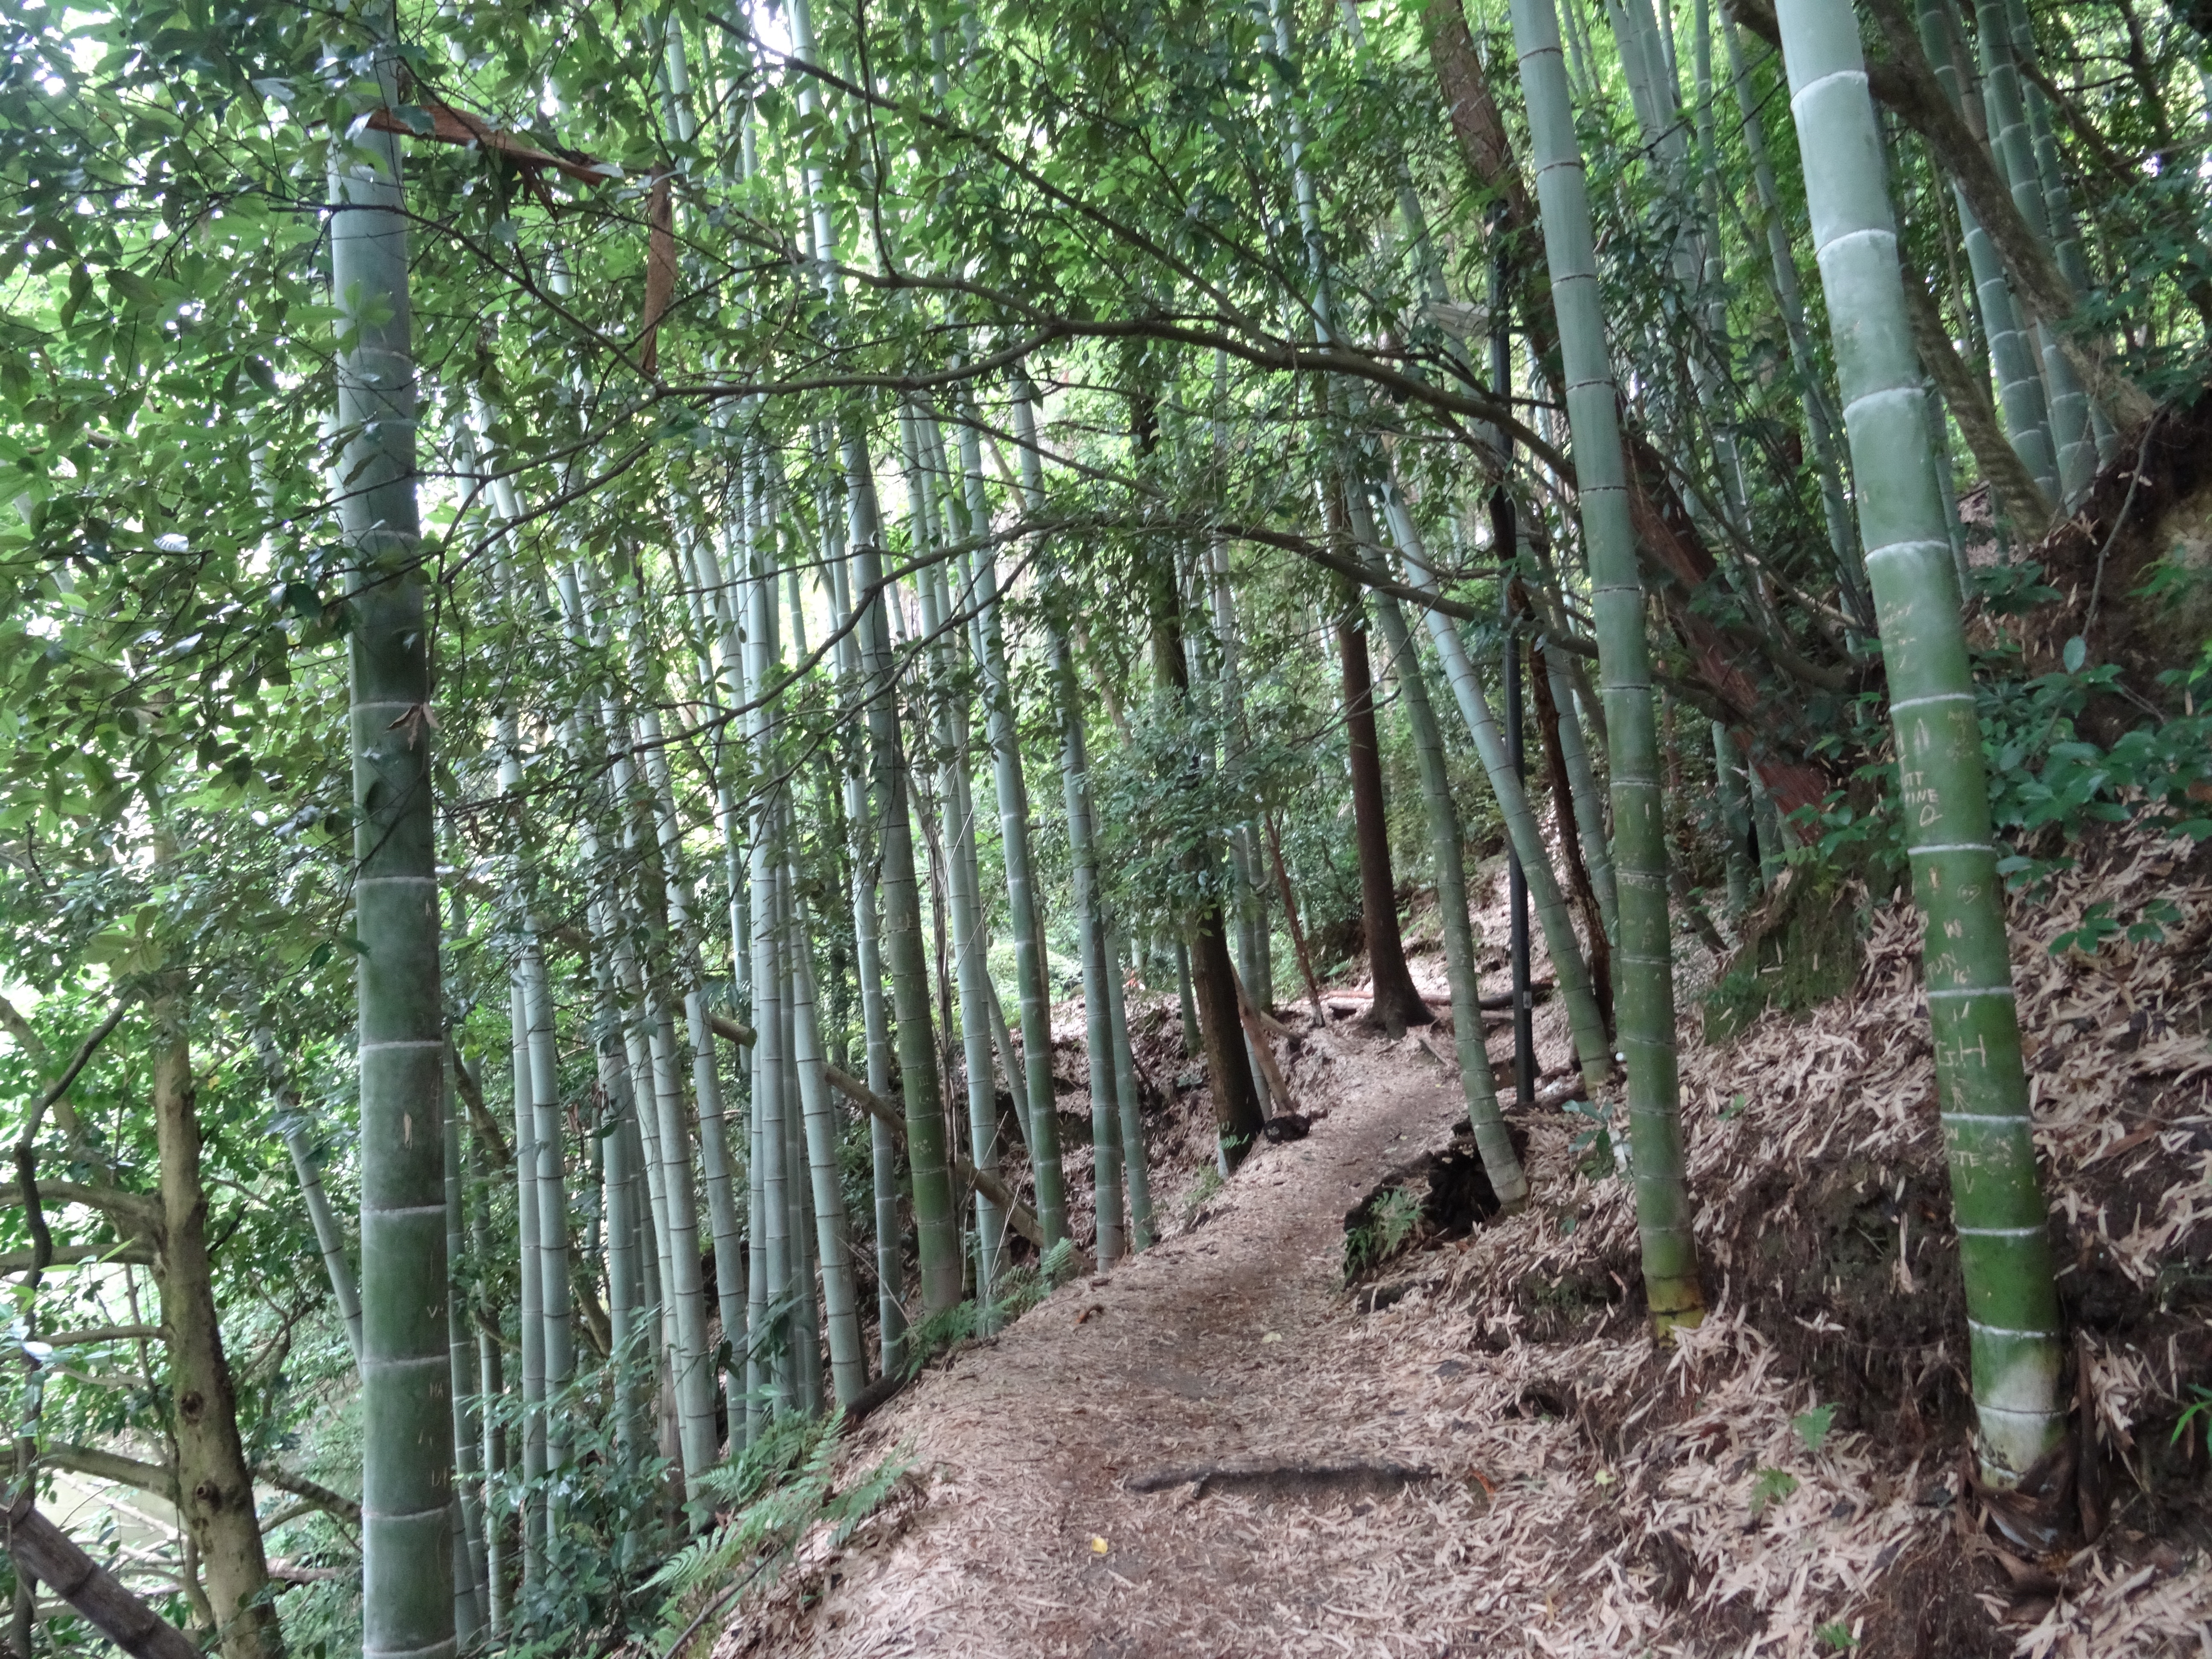
\includegraphics[height=0.3\textheight]{images/DSC03653.JPG}
				\vspace{-3cm}
				\begin{flushright}
					\includegraphics[height=0.3\textheight]{images/IMG_20230208_095155.jpg}
				\end{flushright}
				\vspace{0.5cm}
				\begin{flushleft}
					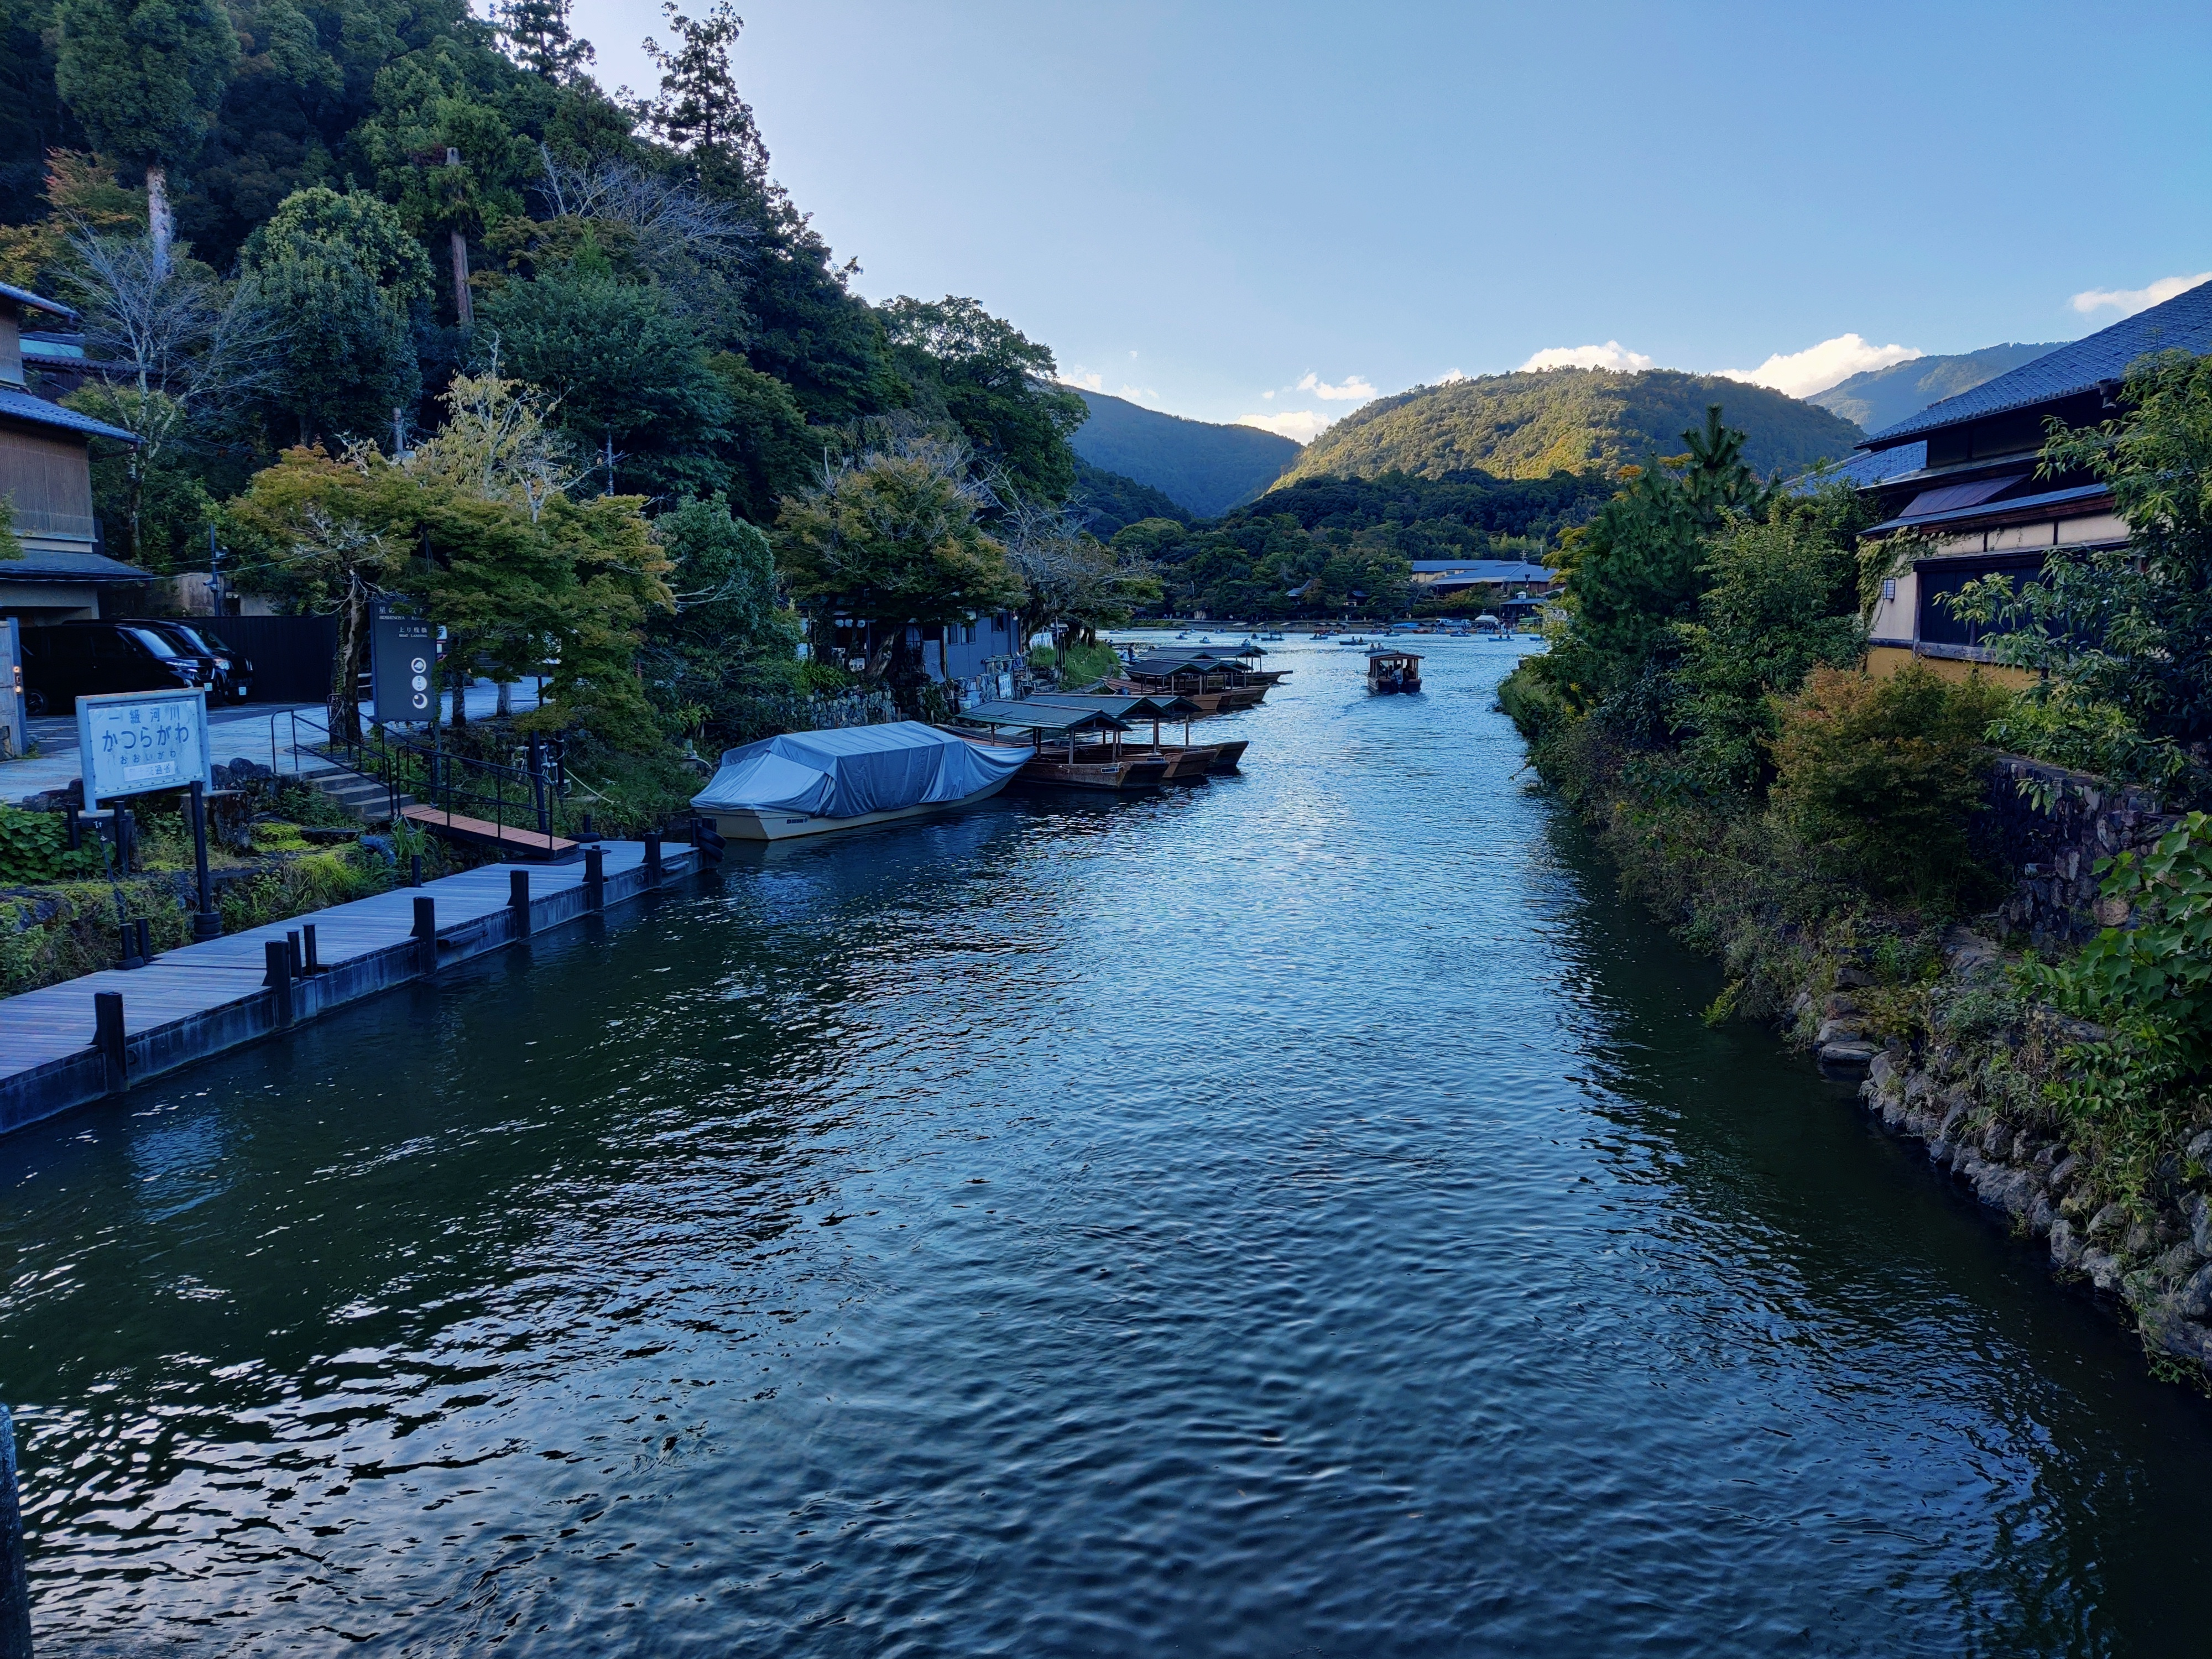
\includegraphics[height=0.3\textheight]{images/IMG_20221008_161529.jpg}
				\end{flushleft}
				\vspace{-3cm}
				\begin{flushright}
					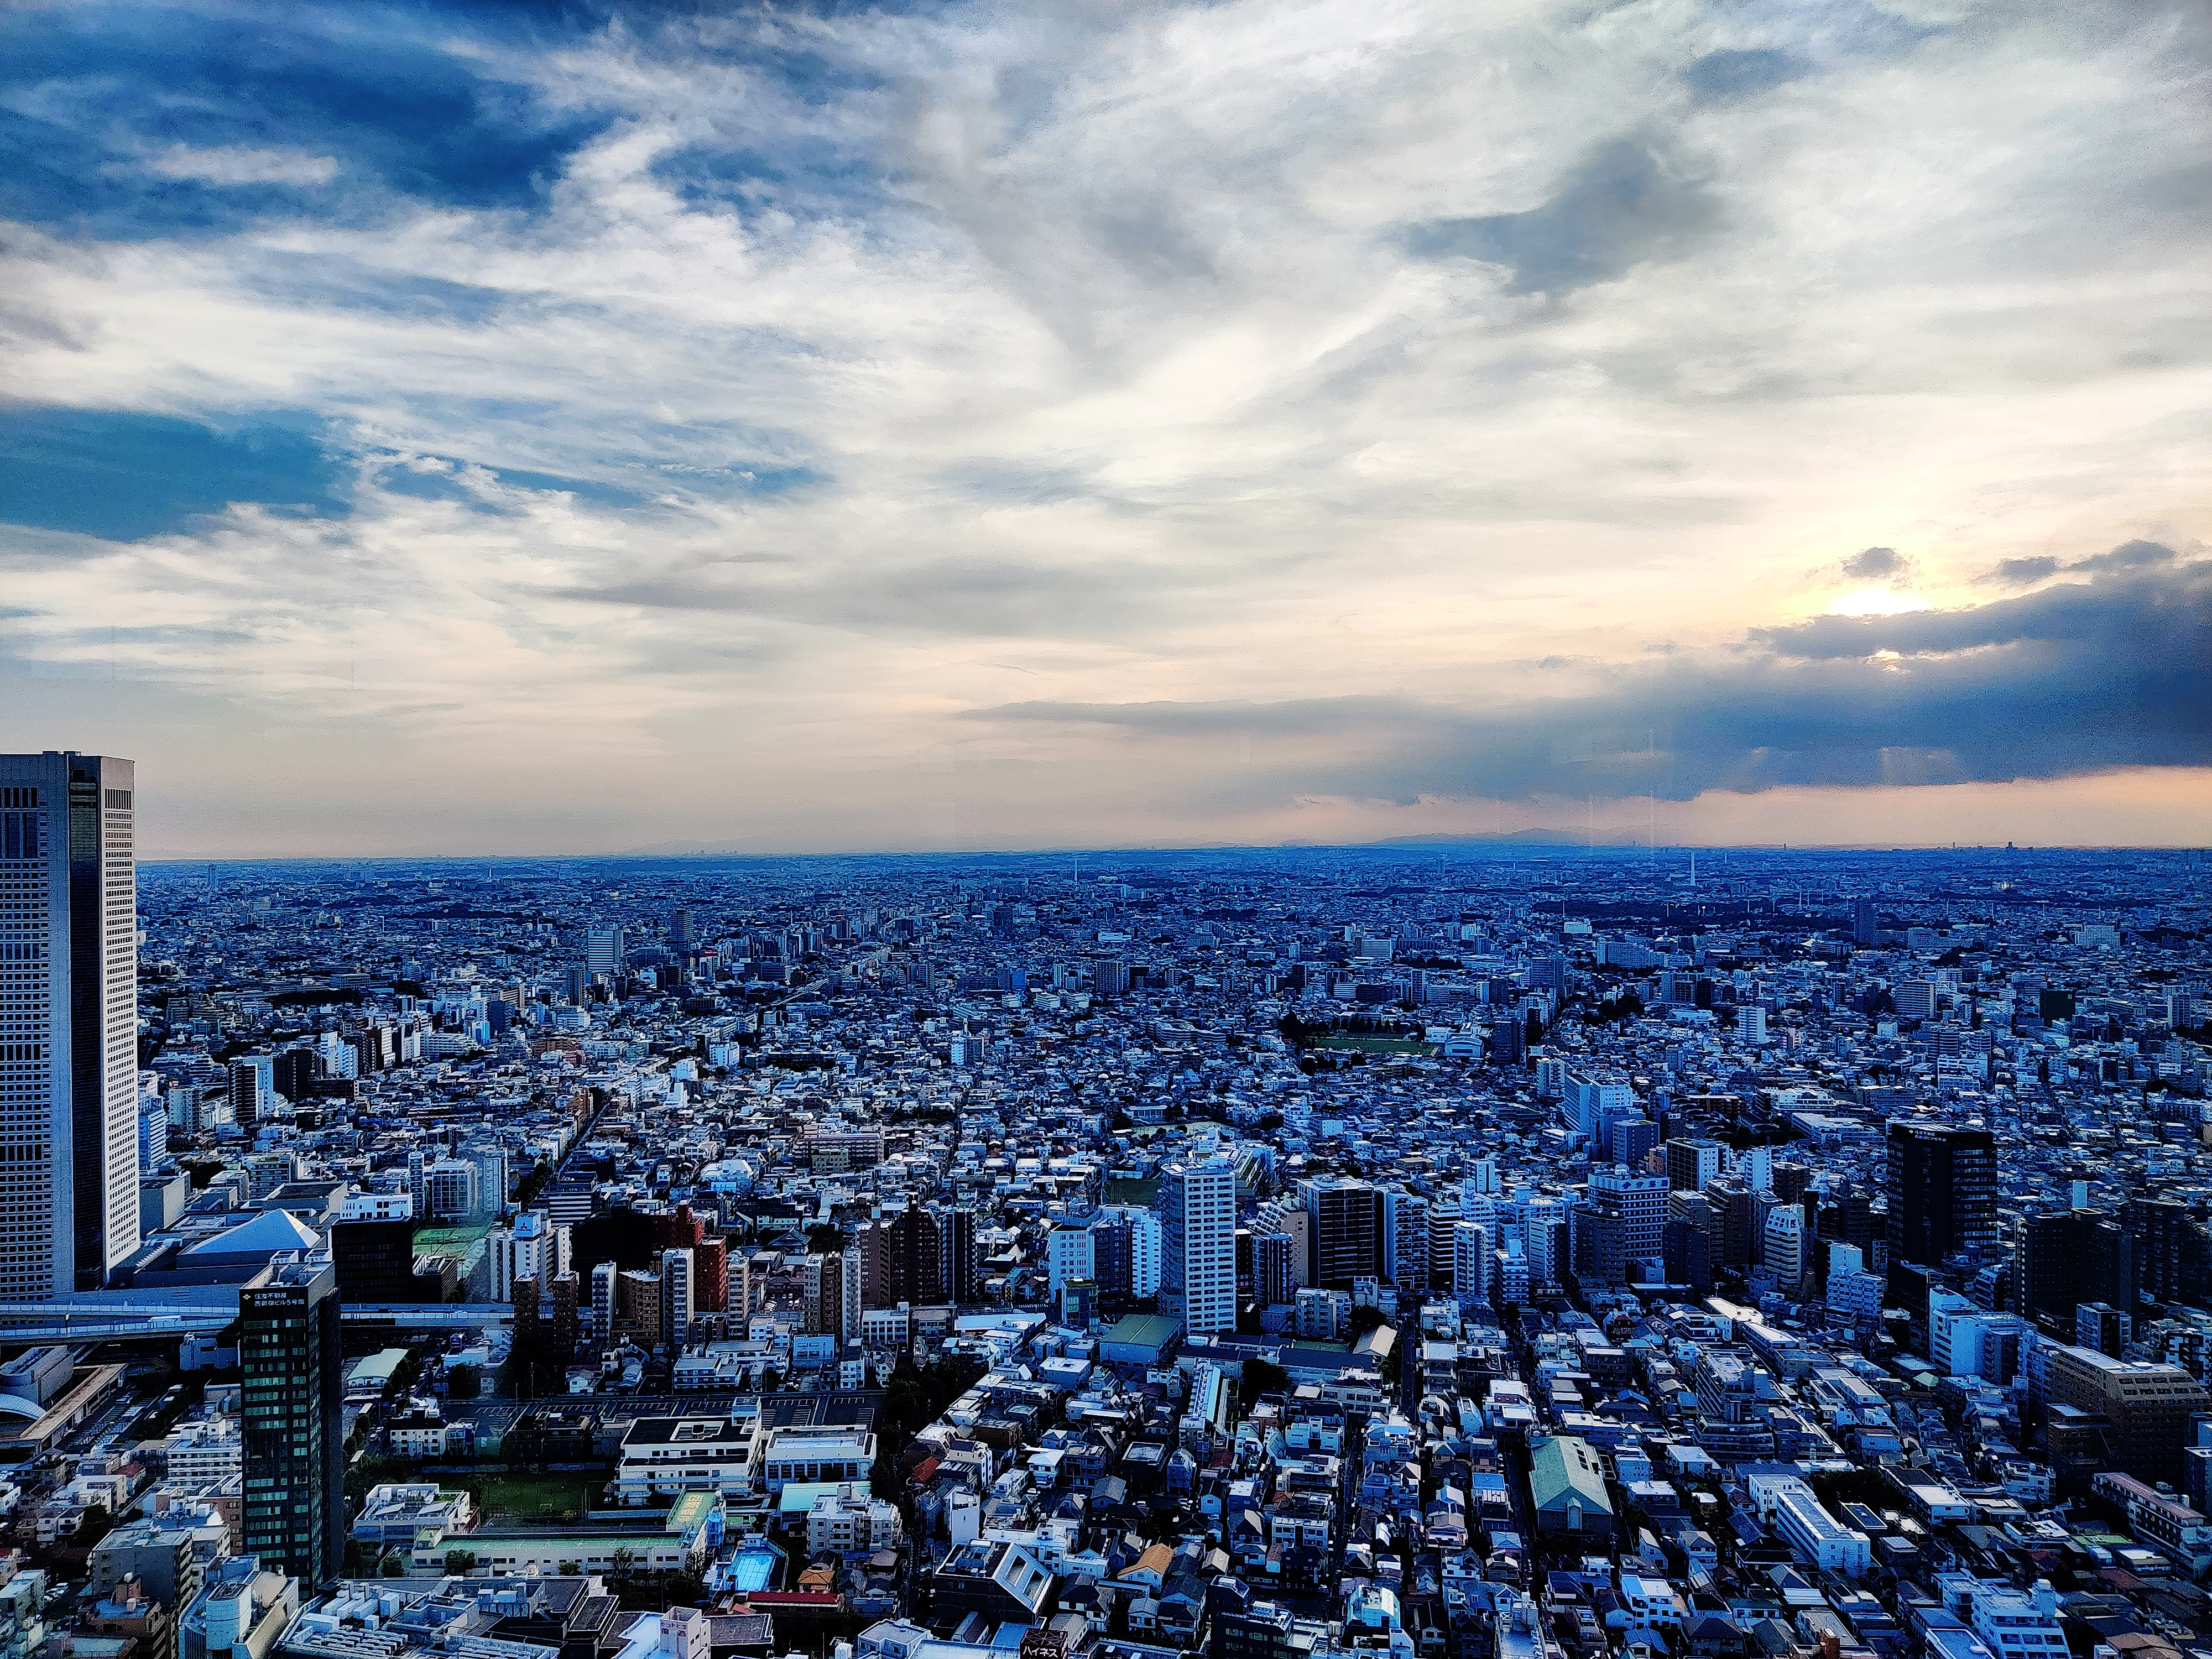
\includegraphics[height=0.3\textheight]{images/IMG_20220913_171859.jpg}
				\end{flushright}}
			\only<8>{
			\includegraphics[height=0.4\textheight]{images/laufstrecke_rund.jpg}
			\vspace{-3cm}
				\begin{flushright}
					\includegraphics[height=0.4\textheight]{images/laufstecke_uturn.jpg}
				\end{flushright}
				%				\vspace{0.5cm}
				\begin{flushleft}
					\includegraphics[height=0.3\textheight]{images/laufstrecke_komplex.jpg}
				\end{flushleft}}
		\end{minipage}
	\end{frame}
	
	\section{Ziel}
	\begin{frame}
		\vspace{0.25cm}
		Was ist das Ziel?
		\pause
		\begin{itemize}[<+->]
			\item Grundlage: Tour4Me
			\item App erweitern und nutzbarer machen
		\end{itemize}
		\pause
		\begin{columns}
			\begin{column}{0.48\textwidth}
				\begin{block}{ Mögliche algorithmische Erweiterungen: Metaheuristiken}		
					\pause			
					\begin{itemize}[<+->]
						\item AntColony
						\item Simulated Annealing
						\item Genetisch
						\item Kombinationen
					\end{itemize}
				\end{block}
			\end{column}
			\pause
			\begin{column}{0.48\textwidth}
				\begin{block}{Mögliche UI Erweiterungen: Mehr Parameter, Änderung des Interfaces}
					\pause
					\begin{itemize}[<+->]
						\item Einbeziehen der genannten Faktoren
						\item algorithmisch und in der GUI
						\item Anpassen der GUI auf neue Optionen
					\end{itemize}
				\end{block}
			\end{column}
		\end{columns} ~\\
		
		\pause
		$\Rightarrow$ allgemein: Tour4Me so anpassen, dass für (fast) jeden Startpunkt und jede Routenlänge ein (möglichst gutes) Ergebnis ausgegeben wird
	\end{frame}
	
	\begin{frame}{Tour4Me Demo}
		\centering
		\vspace{2cm}
		\Huge \href{http://tour4me.cs.tu-dortmund.de/} {Tour4Me}
	\end{frame}
	
	
	\section{Motivation und Hintergrund}	
	\begin{frame}
		\vspace{0.5cm}
		Viele Algorithmen, Ansätze und viel  Forschung zu Kürzeste-Wege-Problemen
		\pause
		\begin{itemize}[<+->]
			\item Reviews, Vergleiche und Analysen \cite{madkourSurveyShortestPathAlgorithms2017, sommerShortestpathQueriesStatic2014, wayahdiGreedyAStarDijkstra2021}
			\item Zusätzlich weitere heuristische Ansätze
			\begin{itemize}[<+->]
				\item local search Varianten \cite{braysyVehicleRoutingProblem2005, irnichSequentialSearchIts2006, ropkeHeuristicExactAlgorithms2005}
				\item neighborhood basierte Ideen \cite{braysyVehicleRoutingProblem2005, irnichSequentialSearchIts2006, ropkeHeuristicExactAlgorithms2005}
			\end{itemize} 
		\item algorithmische Routing-Probleme  bereits NP-schwer \cite{reineltTravelingSalesmanComputational2003}
		\begin{itemize}[<+->]
			\item Traveling Salesman (TSP)\cite{gendreauHandbookMetaheuristics2010} 
			\item vehicle routing \cite{braysyVehicleRoutingProblem2005, irnichSequentialSearchIts2006}
		\end{itemize}
		\end{itemize}
		\pause
		
		$\Rightarrow$ Rundtrips mit Nebenbedingungen noch komplexer \cite{gemsaEfficientComputationJogging2013}
		\pause
		\begin{itemize}[<+->]
			\item vorhandene Tools meist eingeschränkt
			\item Auswahl an Nebenbedingungen beschränkt
			\item Editieren schwierig/ ignoriert Nebenbedingungen
		\end{itemize}
	\end{frame}
	
	\begin{frame}{Beispiele}
		\centering
		\vspace{2.5cm}
		\Huge
		\only<1> {\href{https://www.routeyou.com}{RouteYou}}
		\only<2> {\href{https://www.routeloops.com/}{RouteLoops}}
	\end{frame}
	
	
	\section{Vorgehensweise}		
	\begin{frame}	
		\vspace{0.5cm}
		\begin{block}{}
			\begin{itemize}[<+->]
				\item Interface zum Testen neuer Ansätze und Metaheuristiken (C\#)
				\item Einbauen neuer Auswahloptionen für User (z.B. Höhe/Anstieg)
				\item Implementieren verschiedener Ansätze
				\begin{itemize}[<+->]
					\item Metaheuristiken
					\item Kombinationen dieser
					\item Kobination mit bereits implementierten Ansätzen
				\end{itemize}
				\item Auswertung und Vergleich der Ansätze
				\item Anpassen des User Interfaces
				\item Auswahl des/der best passenden Umsetzungen
				\item Übertragen in eine finale Tour4Me Anwendung (vollständig c++ oder \#)
			\end{itemize}
		\end{block}
	\end{frame}
	
	\begin{frame}{Timeline}
		\centering
		\vspace{0.5cm}
		\tikzstyle{descript} = [text = black,align=center, minimum height=1.8cm, align=center, outer sep=0pt,font = \footnotesize]
		\begin{tikzpicture}[very thick, black]
			\small
			
			%% Coordinates
			\coordinate (O) at (-1,0); % Origin
			\coordinate (P1) at (1,0);
			\coordinate (P2) at (8,0);
			\coordinate (P3) at (11,0);
			\coordinate (P4) at (12.5,0);
			\coordinate (F) at (13,0); %End
			\coordinate (E1) at (5,0); %Event
			\coordinate (E2) at (0.5,0); %Event
			
			
			%% Arrow
			\draw[->] (O) -- (F);
			%% Ticks
			\foreach \x in {0,2,...,12}
			\draw(\x cm,3pt) -- (\x cm,-3pt);
			%% Labels
			\foreach \i \j in {0/Nov,2/Dec,4/Jan,6/Feb,8/Mar,10/Apr,12/May}{
				\draw (\i,0) node[below=3pt] {\j} ;
			}
			\pause
			
			%% Filled regions
			\fill[color=ColorOne!20] rectangle ($(O)+(0.2,0)$) -- (P1) -- ($(P1)+(0,1)$) -- ($(O)+(0.2,1)$);
			\path [pattern color=ColorOne!80, pattern=north east lines, line width = 1pt, very thick] rectangle ($(O)+(0.4,0)$) -- ($(O)+(2,0)$) -- ($(O)+(2,1)$) -- ($(O)+(0.4,1)$);
			\draw ($(P1)+(-0.9,0.5)$) node[activity,ColorOne] {Pre-work};
			\pause	
			
			%% Description
			\node[descript,fill=ColorOne!15,text=ColorOne](P0) at ($(P1)+(2,-2.5)$) {%
				literature\\
				examples\\
				implementing interface};
			
			%% Arrows
			\path[->,color=ColorOne] ($(P1)+(-0.5,-0.1)$) edge [out=-90, in=130]  ($(P0)+(0,1)$);
			\pause
			
			\fill[color=ColorTwo!15] rectangle (P1) -- (P2) -- ($(P2)+(0,1)$) -- ($(P1)+(0,1)$);
			\draw ($(P2)+(-3.55,0.5)$) node[activity,ColorTwo] {Implementing and testing different algorithms,\\ changing other aspects of the app};
			\pause
			
			\fill[ColorThree!30] rectangle (P2) -- (P3) -- ($(P3)+(0,1)$) -- ($(P2)+(0,1)$);
			\draw ($(P3)+(-1.55,0.5)$)  node[activity, ColorThree] {Gathering \\results};
			\pause
			
			\fill[ColorFour!20] rectangle (P3) -- (P4) -- ($(P4)+(0,1)$) -- ($(P3)+(0,1)$);
			\draw ($(P4)+(-0.8,0.5)$)  node[activity, ColorFour!80!black] {Writing \\only};
			\pause
			
			
			%% Events
			\draw [decorate,decoration={brace,amplitude=6pt}]($(P1)+(-1.8,1.2)$) -- ($(F)+(-0.5,1.2)$) node [black,midway,above=6pt, align=center] {Writing on the thesis};
			
			
		\end{tikzpicture}
	\end{frame}
	
	
	\section{Literatur}
	\begin{frame}[allowframebreaks]{Literatur}
		\tiny
		\bibliography{LS11Buchin.bib}
	\end{frame}
	
	
	%*************************************************************
	\begin{frame}{Beispiel Box}
		\begin{block}{\href{https://icpc.global/}{International Collegiate Programming Contest (ICPC)}}
			\begin{itemize}
				\item Association for Computing Machinery (ACM)
				\item seit 1970
				\item an Universit\"uten weltweit
			\end{itemize}
		\end{block}
		\begin{itemize}
			\item Teams von 3 Studierenden
			\item 10 Probleme mit verschiedenem Schwierigkeitsgrad
			\item 1 Computer pro Gruppe
			\item Hilfsmittel: \glqq Cheat Sheet\grqq
			\item L\"osungen werden zu einem Judge Server hochgeladen
			\item Gewinner: die Gruppe, welche die meisten Probleme gel\"ost hat
		\end{itemize}
		
	\end{frame}
	
	
	%*************************************************************
	\begin{frame}{Beispiel column plus Box}
		\vspace{-0.5cm}
		\begin{columns}
			\begin{column}{.65\linewidth}
				\begin{itemize}
					{\small
						\item { \bf 11.10.} Einf\"uhrungstreffen
						\item { \bf 18.10.} Systemeinf\"uhrung
						\item { \bf 25.10.} Tipps und Tricks
						\item { \bf 08.11.} Datenstrukturen und Algorithmenentwurfsmethoden
						\item { \bf 15.11.} Such- und Sortieralgorithmen
						\item { \bf 22.11.} Dynamisch Programmieren
						\item { \bf 29.11.} Strings
						\item { \bf 06.12.} \"Ubungswettbewerb 1
						\item { \bf 13.12.} Graphtraversierung
						\item { \bf 20.12.} Flussalgorithmen und Matchings
						\item { \bf 10.01.} Algorithmische Geometrie
						\item { \bf 17.01.} \"Ubungswettbewerb 2
						\item { \bf 24.01.} Wintercontest oder Interner Wettbewerb 
					}
				\end{itemize}
			\end{column}
			\begin{column}{.25\linewidth}
				\begin{block}{W\"ochentliche Treffen}
					12:15 -- ca.\ 13:30\\
					Besprechung, Vortrag\\
					13:30 -- 15:45\\
					Probleme l\"osen, Hilfestellung
				\end{block}
			\end{column}
		\end{columns}
		
	\end{frame}
	%*************************************************************
	\begin{frame}{Beispiel Spalten mit Boxen}
		\begin{columns}
			\begin{column}{0.3\textwidth}
				\begin{block}{Kommunikation}
					\begin{enumerate}
						\item Sprache
						\item Stimme \& K\"orpersprache
						\item Einfachheit \& Pr\"ogranz, Zeit
					\end{enumerate}
				\end{block}
			\end{column}
			\pause
			\begin{column}{0.3\textwidth}
				\begin{block}{Methodik}
					\begin{enumerate}
						\item Struktur
						\item Stimulanz
						\item Medien- \& Materialeinsatz
						\item Interaktion
					\end{enumerate}
				\end{block}
			\end{column}
			\pause
			\begin{column}{0.3\textwidth}
				\begin{block}{Vortragsqualit\"at}
					\begin{enumerate}
						\item Korrektheit \& Technische Tiefe
						\item Beantowrtung der Fragen
						\item Pr\"asentationsziel
					\end{enumerate}
				\end{block}
			\end{column}
		\end{columns} ~\\
		Motivation beim Vortrag!
	\end{frame}
	%*************************************************************
	\begin{frame}{Thema 1: Datenstrukturen und Algorithmenentwurfsmethoden}
		\begin{columns}
			\begin{column}{0.5\textwidth}
				\begin{itemize}
					\item Listen
					\item Arrays
					\item Stacks
					\item Heaps
					\item Hashing
				\end{itemize}
			\end{column}
			% \end{frame}
		% %*************************************************************
		% \begin{frame}{Thema 2: }
			\begin{column}{0.5\textwidth}
				\begin{itemize}
					\item Greedy
					\item Divide \& Conquer
					\item Brute-Force
					\item Backtracking
				\end{itemize}
			\end{column}
		\end{columns}
	\end{frame}
	
	%*************************************************************
	
	%*************************************************************
	%*************************************************************
\end{document}

